% Zuhayr Loonat - University of Cape Town - LNTZUH001

% This is a project report templace document created for EEE4022FS students at the University of Cape Town.
%
% This file should be is processed with ``pdflatex`` and might need a few modifications if a different processor is chosen.


\documentclass[a4paper,12pt]{report}

%Include packages you need to use here

\usepackage[top = 1in, bottom = 1in, left = 1in, right = 1in]{geometry}
\usepackage{graphicx}
\usepackage{fancyhdr}
\usepackage{amsmath, amsthm, amssymb}
\usepackage{lastpage}
\usepackage{subfigure}
\usepackage{lscape}
\usepackage{hyphenat}
\usepackage{setspace}
\usepackage{hyperref}

% Include page formatting here. 
\parskip = 6mm
\parindent = 0mm
\renewcommand{\headrulewidth}{0pt}
\rhead[]{\thesection}
\lhead[\thechapter]{}


\begin{document}

% This section formats the title page of the Report.
\thispagestyle{empty}
    {\Huge \begin{center}
        % Modify the line below to insert your title.
        Measurement of Water Salinity \\in Water Towers
        %\hrule 
        % Modify the line below to insert your subtitle.
        %{\Large Insert a subtitle here (if applicable)}
    \end{center}}

    \vskip 5mm
    \begin{center}
        
\includegraphics[scale = 0.35]{Figures/uctLogo.png}
    \end{center}

    \vskip 5mm
    \begin{center}
        Presented by:\\
        Zuhayr Loonat		% Insert your name here
    \end{center}

    \vskip 10mm
    \begin{center}
        Prepared for:\\
        Justin Pead\\ 		% Insert your supervisor's name here.
        Dept. of Electrical Engineering\\University of Cape Town
    \end{center}


    \vskip 10mm
    \begin{center}
        Submitted to the Department of Electrical Engineering at the University of Cape Town in partial
        fulfilment of the academic requirements for a Bachelor of Science degree in Electrical and Computer Engineering
    \end{center}


    \vskip 5mm
    \begin{center}
        {\bf \today}
    \end{center}

%second Page
%\newpage
%\thispagestyle{empty}
%\mbox{}

% Declarartion
\fancyfoot[C]{\thepage}
\pagestyle{plain}
\newpage
\pagenumbering{roman}
%\newpage
    \onehalfspacing
    \nohyphens{
    %\thispagestyle{empty}
    \vskip 40mm


    % Please leave the declaration as it is (Standard UCT declaration).
    {\Huge Declaration}\\
    %\hrule

    \vskip 10mm
    \begin{enumerate}
        \item I know that plagiarism is wrong.
        Plagiarism is to use another’s work and pretend that it is one’s own.
        \item I have used the IEEE convention for citation and referencing.
        Each contribution to, and quotation in, this report `The Measurement of Water Salinity in Water Towers' from the work(s) of other people has been attributed and has been cited and referenced.
        Any section taken from an internet source has been referenced to that source.
        \item This report `The Measurement of Water Salinity in Water Towers' is my own work and is in my own words (except where I have attributed it to others).
        \item I have not paid a third party to complete my work on my behalf.
        My use of artificial intelligence software has been limited to giving overviews of topics, aiding with \LaTeX commands, and aiding with making BibTeX citations of sources (specify precisely how you used AI to assist with this assignment, and then give examples of the prompts you used in your first appendix).
        \item I have not allowed and will not allow anyone to copy my work with the intention of passing it off as his or her own work.
        \item I acknowledge that copying someone else’s assignment or essay, or part of it, is wrong, and declare that this is my own work
    \end{enumerate}
    \vskip30mm
        \begin{tabular*}{\textwidth}{@{}l@{\extracolsep{\fill}}r@{}}
        Signature:\ldots\ldots\ldots\ldots\ldots\ldots\ldots\ldots\ldots & Date: {\today} \\
        Zuhayr Loonat & \\
        \end{tabular*}
        \vskip10mm

\newpage
    %\thispagestyle{empty}
    {\Huge Terms of Reference}\\
    %\hrule
    \vskip 10mm
    The terms of reference page is an agreement between yourself and your supervisor outlining what is expected of you in your final year project. Please make sure that this is discussed and written at the beginning of your thesis project. 


%\fancyfoot[C]{\thepage}
%\pagestyle{plain}
%\pagenumbering{roman}
\newpage
{\Huge Acknowledgments}\\
%\hrule
\vskip 10mm
Make relevant acknowledgements to people who have helped you complete or conduct this work, including sponsors or research funders.


\newpage
    {\Huge Abstract}\\
    %\hrule
    \vskip 10mm

    % Place your abstract here.
    \begin{itemize}
        \item Open the {\bf Project Report Template.tex} file and carefully follow the comments (starting with \%).
        \item Process the file with {\bf pdflatex}, using other processors may need you to change some features such as graphics types.
        \item Note the files included in the  {\bf Project Report Template.tex} (with the .tex extension excluded). You can open these files separately and modify their contents 
        or create new ones.
        \item Contact the latex namual for more features in your document such as equations, subfigures, footnotes, subscripts \& superscripts, special characters etc.
        \item I recommend using the {\bf kile} latex IDE, as it is simple to use.
    \end{itemize}


\newpage
    \tableofcontents

%\newpage
%\listoffigures

%\newpage
%\listoftables

% Page formatting, to place section titles as headers of odd pages and Chapter titles as headers of even pages.
\newpage
\fancyhead[RE,LO]{}
\fancyhead[LE]{\leftmark}
\fancyhead[RO]{\rightmark}
\pagestyle{fancy}

\pagenumbering{arabic}

% THe files included below are .tex files containing the respective chapters these are already created in this package and you can add to or modify them.
\chapter{Introduction}

\section{Background to the study}
A very brief background to your area of research. Start off with a general introduction to the area and
then narrow it down to your focus area. Used to set the scene\cite{smt2011}.
\section{Objectives of this study}
\subsection{Problems to be investigated}
Description of the main questions to be investigated in this study.
\subsection{Purpose of the study}
Give the significance of investigating these problems. It must be obvious why you are doing this study
and why it is relevant.

\section{Scope and Limitations}
Scope indicates to the reader what has and has not been included in the study. Limitations tell the
reader what factors influenced the study such as sample size, time etc. It is not a section for excuses as
to why your project may or may not have worked.

\section{Plan of development}
Here you tell the reader how your report has been organised and what is included in each
chapter.

{\bf I recommend that you write this section last. You can then tailor it to your report.}

\chapter{Literature Review}
\section{Introduction}
Accurate salinity measurement is fundamental to oceanographic research.
Traditional measurement techniques have evolved from labour-intensive chemical titration methods to modern electronic sensors, with electrical conductivity emerging as the predominant approach due to its combination of accuracy, speed, and practical deployability.
This literature review examines the current state of salinity measurement technology with particular emphasis on conductivity-based methods and emerging machine learning approaches for electrochemical data interpretation. The review is organised into three main sections.
First, we establish the fundamental concepts of salinity and provide a comprehensive comparison of available measurement techniques.
Second, we examine the theoretical foundations and practical implementation of electrical conductivity measurements for salinity determination, including instrumentation, calibration procedures, and current limitations.
Finally, we explore the application of \gls{eis} and \gls{ml} as advanced approaches for enhanced salinity analysis, examining how frequency-domain measurements and intelligent data processing can overcome limitations of traditional single-frequency conductivity methods.
This comprehensive review provides the theoretical and methodological foundation for developing a machine learning-enhanced impedance spectroscopy approach for salinity determination.

\section{Salinity: Definition}
Salinity is a fundamental characteristic of water, and is most commonly defined as the total amount of dissolved salts in water, and in the context of oceanography, seawater.
It is typically expressed in \gls{ppt} or \gls{psu}~\cite{salinity_def}. 
The concept of salinity has evoloved significantly from its early definition, which was based on chlorinity measurements.
Modern salinty is defined through the Practical Salinity Scale 1978 (PSS-78), where salinity is based on the conductivity ratio of standard seawater solutions, to a standard Potassium Chloride solution, and is dimensionless~\cite{unesco_salinity}.
The salinity-conductivity relationship is however, quite complex, requiring corrections and calibrations needed for depth and temperature, as these both play a factor in the conductivity of the water. 

\section{Overview of Salinity Measurement Methods}
There are a multitude of methods which can be used to measure salinity, each with their own advatages, limitations and levels of accuracy.
Traditional methods include gravimetric analysis, chemical titration (such as the Mohr-Knudsen method for chlorinity), and refractometry. While these techniques can provide accurate results, they are often time-consuming, require skilled operators, and are not easily adaptable to in-situ or automated measurements.
Modern approaches predominantly rely on electrical conductivity sensors, which offer rapid, repeatable, and automated salinity determination.
Other techniques, such as optical methods and ion-selective electrodes, have also been explored, but are less commonly used in oceanographic applications due to issues with robustness, calibration, or specificity.
The choice of method depends on the required accuracy, operational environment, and available resources.


\subsection{Historical Methods}
\subsubsection{Chlorinity Titration}
Early salinity measurements relied on chemical titration methods, in particular the Mohr-Knudsen chlorinity titration, which used silver nitrate.
The chlorinity of a solution has the definition `the mass of silver required to precipitate completely the halogens in $0.3 285 234 kg$ of sample seawater'.
This method was highly accurate, with results within ($\pm0.001$ PSU). However, it relied heavily on toxic chemicals, and was a time-consuming laboratory procedure, with limited practical application in the field~\cite{lewis_pss78}.

\subsubsection{Gravimetric Methods}
Gravimetric analysis, a technique used to determine an amount of a substance, by measuring its change in mass, invloves evaporation and the weighing of dissovled solids.
This method directly provided measurements of the salt content, within accuracies of ($\pm0.001$ PSU), under controlled laboratory conditions.
This method remains the reference standard for calibration processes, but is however, extremely slow~\cite{chemical_ocean}.

\subsection{Physical Property Based Methods}
There are several methods that utilise the relationship between salinity and the physical properties of water.

\subsubsection{Hydrometric and Density Methods}
Hydrometric methods using density measurements via hydrometers, offer salinity measurements that are low-cost, and electronics free. 
However, they are limited in precision with accuracies of $\pm 1-2$ PSU, and require large sample volumes.
The hydrometer is a floating instrument, that sinks to different depths depending on the density of the solution, and by measuring how high or low it floats, the density of the solution can be determined~\cite{the_globe_program_hydrometer}.
The following equation is used to map the relationship between salinity and density~\cite{kjerfve_density}.

\begin{equation}
    \rho = \rho_0(1+kS)
\end{equation}

where $\rho$ is the density, $\rho_0$ is the density of fresh water, $S$ is the salinity and $k$ is the proportionality constant. 

This can then be inverted to give Salinity from Density:

\begin{equation}
S = \frac{\frac{\rho}{\rho_0}-1}{k}
\end{equation}

This however, does not include temperature correction.

\subsubsection{Refractometric Thechniques}
Refractometric techniques measure the refractive index changes cuased by the dissovled salts.
The refractive index of seawater is influenced by wavelength, temperature, salinity, and pressure. 
Within the range of 500-700~nm wavelength, 0-30$^\circ$C temperature, 0-40~PSU salinity, and 0-11000~dbar pressure, the refractive index equation provides an accuracy of 0.4-80~ppm~PSU, with accuracy decreasing as pressure increases~\cite{refraction_millard}.
Refractometers, which require only a small sample volume, are compact devices, making them suitable for portable field measurements~\cite{malarde_high-resolution_refractometer}.
Fibre optic refractometers have improved portability and reduced temperature sensitivity, with moderate accuracy (±0.5-1 PSU), making them increasingly popular in aquaculture applications~\cite{zhang_high-temperature_fibre}. 


\subsubsection{Freezing Point Osmometry}
Freezing point depression osmometry exploits the colligative (i.e.~relating to the binding together of molecules) properties of dissolved salts.
The main principle relies on freezing point depression, which is the phenomenon where a solvents freeving point is lowered when a solute is added to it.
To perform the measurement, the water is cooled till its freezing point and the temperature drop is measured, which is then used to calculate the osmolality~\cite{freeze_abele}.
This method can achieve accuracies of $\pm2 mOsm/kg H_{2}O$ which is approximately $\pm0.1-0.2$ \gls{ppt}. However its requirement for precise temperature control limits its usage to laboratory applications~\cite{freezing_accuracy}.


\subsubsection{Magnetic Permeability}
Magnetic properties of liquids, particularly magnetic susceptibility, vary with ion concentration, offering a potential method for salinity determination.
Research has demonstrated that bulk magnetic susceptibility (BMS) of saline water correlates with salinity and conductivity measurements, with water quality parameters exhibiting an inverse relationship with magnetic susceptibility values.
This approach offers the benefit of non-contact measurement, potentially avoiding sample contamination or disturbance~\cite{rana_magnetic_2021}.
However, the technique requires sophisticated instrumentation, which are typically designed for laboratory use rather than field deployment. 



\subsection{Advanced Analytical Methods}
\subsubsection{Ion Chromatography}
Ion chromatography is an analytical technique used to separate and quantify ionic species in solution, making it highly valuable for determining the individual ion concentrations in seawater samples~\cite{ion_chromatography}.
The method works by passing a liquid sample through a column containing special resin beads that selectively hold onto different ions.
As a liquid solution flows through, ions are released at different times based on their properties and detected by measuring electrical conductivity.
For seawater analysis, ion chromatography can separately measure major ions like chloride, sulfate, sodium, magnesium, calcium, and potassium, providing detailed compositional data rather than just total salinity. 
The technique offers high precision and can detect ions at very low concentrations, though it requires more sophisticated equipment and longer analysis times compared to simpler methods~\cite{gros_ionic_2008}.

\section{Conductivity-Based Salinity Measurements}
\subsection{Theoretical Foundation}
Electrical conductivity has emerged as the predominant method for salinity measurement due to its practical implementation, high accuracy and fast response time.
The technique utilises the strong correlation between dissolved ionic content and electrical conductivity.

The conductivity of a liquid is measured by its ability to conduct electrical current.
The relationship between conductivity and salinity is based on the concentration of dissolved ions in seawater.
The main ions found in sea water ($Na^+, Cl^-, Mg^{2+}, {SO_4}^{2-}, Ca^{2+}, K^+$) maintain a relatively constant proportional relationship, in ocean waters~\cite{chemical_ocean}.
This enables robust corrections between conductivity and total dissolved salt content.
Unlike other measurement techniques, conductivity accounts for all the ions in the water, not only chlorine, which is why it is considered a more accurate measure of salinity~\cite{salinity_def_calc}.

The Practical Salinity Scale 1978 (PSS-78) defines Practical Salinity $S_p$ through the conductivity ratio $K_{15}$, as shown below~\cite{teos-10}:

\begin{equation}\label{eqn:k15_salinity}
    K_{15} = \frac{C(S_p, 15, 0)}{C(KCl, 15, 0)}
\end{equation}

where the numerator, $C(S, 15, 0)$ represents the conductivity of seawater sample at 15$^\circ$C and standard atmospheric pressure ($1 atm/101.325 kPa/0dbar$), and the denomimator, $C(KCl, 15, 0)$ is the conductivity of a standard $KCl$ (Potassium Chloride) solution under identical temperature and pressure.
The standard $KCl$ solution consists of $32.4356 \times 10^{-3}kg$ of $KCl$ dissolved in $1kg$ of water~\cite{lewis_pss78}.
When the ratio between the water sample and the $KCl$ solution is 1, i.e. $K_{15} = 1$, then the Practical Salinity $S_p$ is, according to the definition, 35~\cite{teos-10}.

It is important to note that Practical Salinity is a unit-less quantity, and though it may be convenient, it would be incorrect to quote it in \gls{psu}. 
Practical salinity should rather be quoted as a certain Practical Salinity `on the Practical Salinity Scale PSS-78'~\cite{teos-10}. 

When $K_{15}$ does not equal 1, Practical Salinity, $S_p$ can be calculated using the equation below~\cite{teos-10}: 
\begin{equation}\label{eqn:salinity_short}
    S_p = \sum_{i=0}^{5}a_i{(K_{15})}^{i/2} 
\end{equation}

where $K_{15}$ is the equation defined above (Equation~\ref{eqn:k15_salinity}), and the coefficients $a_i$ are given in Table (\ref{tabel:pss-78}).


\subsection{Temperature and Pressure Compensation}
When calculating salinity at conditions other than 15$^\circ$C, and $0dbar$, the conductivity ratio $R$ is expanded to the product of three ratios $R_p$, $R_t$ and $r_t$ as follows~\cite{teos-10}:
\begin{equation}
    R=\frac{C(S_p, t, p)}{C(35, 15, 0)} = R_p R_t r_t
\end{equation}

where $t$, and $p$ are the temperature and pressure valid over the ranges $-2^{\circ}C \leq t \leq 35^{\circ}C$ and $0 \leq p \leq 10 000dbar$ respectively.

These ratios can be expanded as follows:

\begin{equation}
    R = \frac{C(S_p, t, p)}{C(35, 15^{\circ} C, 0)} = \frac{C(S_p, t, p)}{C(S_p, t, 0)} \cdot \frac{C(S_p, t, 0)}{C(35, t, 0)} \cdot \frac{C(35, t, 0)}{C(35, 15^{\circ} C, 0)} = R_p R_t r_t
\end{equation}

This equation represents the ratio between the conductivity measurement of a sample $C(S_p,t,p)$ and the conductivity of the standard solution $C(35, 15^{\circ}, 0)$~\cite{teos-10}. 
In order to find the salinity, $R_p$, $R_t$ and $r_t$ need to be caculated.
First, $r_t$ is calculated using the temperature of the sample:
\begin{equation}
    r_t = \sum_{i=0}^{4} {c_i}{t_i}
\end{equation}
$R_p$ is then calculated as a function of the temperature $t$, pressure $p$, and conductivity ratio $R$:
\begin{equation}
    R_p = 1 + \frac{\sum_{i=1}^{3}{e_i}{p^i}}{1+d_1{t}+d_2{t^2}+R[d_3+d_4 {t}]}
\end{equation}
Finally, $R_t$ can be evaluated using $R$, $R_p$ and $r_t$:
\begin{equation}
    R_t = \frac{R}{{R_p}{r_t}}
\end{equation} 

At standard conditions, i.e., temperature $t=15{^\circ}$C, $R_t$ is equal to $K_{15}$ an therefore Practical salinity $S_p$ can be calculated from Equation~\ref{eqn:k15_salinity}.
For cases where the temperature is not $t=15^\circ$C, Practical Salinity $S_p$ is given as a function of $R_t$, with $k=0.0162$~\cite{teos-10}:
\begin{equation}\label{eqn:salinity_full}
S_p = \sum_{i=0}^{5} a_i {(R_t)}^{i/2} + \frac{t-15}{1+k(t-15)} \sum_{i=0}^{5} b_i {(R_t)}^{i/2}
\end{equation}

Note that Equations~(\ref{eqn:k15_salinity}) to~(\ref{eqn:salinity_full}) are only valid in the range $2 < S_p < 42$, $-2^{\circ}C \leq t \leq 35^{\circ}C$ and $0 \leq p \leq 10 000dbar$.

\begingroup
    \renewcommand{\arraystretch}{1.8} % increase row height (adjust factor as needed)
    \begin{table}[h!]
        \centering
            \begin{tabular}{|>{\centering\arraybackslash}p{1cm}|
                >{\centering\arraybackslash}m{2cm}|
                >{\centering\arraybackslash}m{2cm}|
                >{\centering\arraybackslash}m{3cm}|
                >{\centering\arraybackslash}m{3cm}|
                >{\centering\arraybackslash}m{3cm}|}
            \hline
            $i$ & $a_i$ & $b_i$ & $c_i$ & $d_i$ & $e_i$ \\ \hline
            0 & $0.0080$ & $0.0005$ & $\num{6.766097e-1}$ &  &  \\ \hline
            1 & $-0.1692$ & $-0.0056$ & $\num{2.00564e-2}$ & $\num{3.426e-2}$ & $\num{2.070e-5}$ \\ \hline
            2 & $25.3851$ & $-0.0066$ & $\num{1.104259e-4}$ & $\num{4.464e-4}$ & $\num{-6.370e-10}$ \\ \hline
            3 & $14.0941$ & $-0.0375$ & $\num{-6.9698e-7}$ & $\num{4.215e-1}$ & $\num{3.989e-15}$ \\ \hline
            4 & $-7.0261$ & $0.0636$ & $\num{1.0031e-9}$ & $\num{-3.107e-3}$ &  \\ \hline
            5 & $2.7081$ & $-0.0144$ &  &  &  \\ \hline
            \end{tabular}
        \caption{Table of Coefficients for PSS-78 Equations~\cite{teos-10}}
        \label{tabel:pss-78}
    \end{table}
\endgroup

It must be noted that the PSS-78 equations use the IPTS-68 temperature scale and in order for them to work with the current ITS-90 scale, must be converted using the equation below~\cite{teos-10}:
\begin{equation}
    t_{68}^{\circ}C = 1.00024\times{t_{90}^{\circ}C}
\end{equation}


\subsection{Instrumentation and Technology}
The most common method for measuring salinity is by using a~\gls{ctd} device.
The fundamental concept of these devices involves placing two electrodes in a sample of water, applying a voltage across them and measuring the water's response. This is then paired with a temperature and depth correction, allowing for an accurate salinity measurement.
The depth value for these calculations is taken from the pressure at which the measurement is taken.
This pressure is then translated to depth using the standard depth to pressure equation~\cite{chip_based_ctd}.
Modern CTD systems achieve salinity accuracies better than $\pm0.005$ \gls{psu}, with some instruments like the Sea-Bird 911 Plus demonstrating historical accuracies of $\pm0.002$ \gls{psu} or $\pm0.0002$ \gls{psu}~\cite{chip_based_ctd}~\cite{ctd_accuracy}.

\subsection{Applications and Limitations}
Conductivity-based salinity measurements excel in most oceanographic and water quality applications due to its accuracy, speed, and reliability.
The conductivity method allows for real-time data capture, continuous monitoring, and easy integration with autonomous devices~\cite{roemmich_argo_2009}. 

However, this method does face some limitations. Due to its dependance on the water's capacity to conduct electricity, freshawater applications require specialised low-conductivity sensors, while hyper-saline environments could exceed the standard calibration range.
The method's reliance on emperical correlations derived from typical seawater compositions can introduce errors in waters ocean waters affected by external factors such as pollution or freshwater inflow from connecting rivers, which can alter ionic composition and introduce variability not captured by standard seawater-based calibrations.
In such environments supplementry practices may be necessary for accurate salinity measurements~\cite{uncles_estuarine_2002}.

\section{Machine Learning Applications in Electrochemical \\ Impedance Spectroscopy}
\subsection{Electrochemical Impedance Spectroscopy (\gls{eis})}

\glsfirst{eis} is an analytical technique used to characterise the electrical properties of materials and interfaces, usually electrode or an electrolyte, by measuring impedance (opposition to current flow) across a range of frequencies~\cite{canales_electrochemical_2021}.
In essence, EIS describes the electrode behavior in the presence of an electrolyte in terms of electrical parameters, including resistances and capacitances.
It involves measuring the system's response to an applied electrical signal, and then transforming these time-domain signals into the frequency domain.
The technique is based on applying an /gls{ac} signal to the electrodes and determining the corresponding response.
Unlike simple conductivity measurements that capture only resistive properties at a single frequency, EIS measures both the magnitude and phase of impedance across a range of frequencies, typically from 0.001 Hz to 1 MHz~\cite{barsoukov_impedance_2005}.

The complex impedance $Z(\omega)=Z'(\omega)+jZ''(\omega)$ contains both resistive (real) and reactive (imaginary) components, that respond differently to ionic concentration, species mobility, and electrode interface effects.
High-frequency impedance primarily reflects bulk solution resistance, while lower frequencies reveal interfacial (between two faces) phenomena including double-layer capacitance and charge transfer resistance~\cite{orazem_electrochemical_2008}.

EIS has demonstrated success in quantitative concentration analysis across diverse solution systems.
In electrolyte analysis, multi-frequency measurements enable determination of ionic strength through characteristic impedance signatures that are less sensitive to temperature variations and electrode fouling than DC conductivity measurements~\cite{barsoukov_impedance_2005}.


\subsection{EIS Fundamentals}
The \gls{eis} measuring process invloves applying an AC signal at a specific frequency and amplitude to a sample.
By sweeping across a multitude of frequencies, a complete impedance spectrum can be obtained.
The impedance magnitude $|Z|$ and phase angle $\phi$ at each frequency is recorded, and are used to analyse the electrical properties of the solution~\cite{orazem_electrochemical_2008}.
For salinity, it can be used to characterise the electrical properties of ionic solutions, including seawater, by analyzing how ions affect the impedance spectrum. 
This data can be used to approximate the system using \glspl{eec}, which are circuits ussed to describe a system with discrete electrical circuit elements~\cite{barsoukov_impedance_2005}.
\glspl{eec} fulfill the overall goal of \gls{eis} is to describe the behaviour of the electrode and solution in terms of electrical parameters such as resistances and capacitances~\cite{canales_electrochemical_2021}.

\section{Machine Learning for Impedance to Salinity Mapping}
\subsection{Limitations of Traditional Calibration Approaches}
Traditional impedance analysis relies on the modelling of \glspl{eec}, to derive the salinity from the impedance.
This process requires extensive electrochemical expertise, in order to understand the chemical composition of the solution.
Manual parameter extraction from impedance spectra is time consuming and may fail to capture subtle features that correlate with salinity.
Linear calibration methods assume simple relationships between impedance measurements and concentration, which may not hold across wide salinity ranges or in solutions with varying ionic compositions.
Temperature effects and electrode aging can further complicate traditional calibration approaches~\cite{barsoukov_impedance_2005}.

\subsection{Machine Learning Modelling for Impedance Analysis}
Machine learning approaches offer advantages by learning complex non-linear relationships directly from experimental data without the need for explicit physical models or \glspl{eec}.
Supervised learning algorithms can map measured impedance values at specific input signal frequencies and amplitudes to target salinity concentrations through automated pattern recognition.
The general framework involves training a model on a dataset of known salinity samples, where each sample is characterised by its impedance response to AC excitation at defined frequencies and amplitudes~\cite{bongiorno_exploring_2022}. 
The trained model can then predict salinity from new impedance measurements, effectively learning the impedance-salinity mapping function.
Machine learning eliminates subjective bias inherent in manual impedance interpretation and consistently applies identical analysis procedures across all measurements.
The algorithms can identify complex patterns in multi-frequency impedance data that may be overlooked in traditional analysis~\cite{xu_electrochemical_2020}.

\subsection{Machine Learning Algorithms for Salinity Prediction}
\subsubsection{Neural Networks}
Neural networks are machine learning programs that make decisions similarly to the human brain, using processes that mimic how biological neurons work together to identify patterns, weigh options, and reach conclusions.

Every neural network consists of layers of nodes (artificial neurons), these being an input layer, one or more hidden layers, and an output layer. Each node connects to others and has its own weight and threshold value.
When a node's output exceeds its threshold value, it activates and sends data to the next layer, if not, no data passes through.
This creates a feed-forward process where information flows from input to output. Each node functions like a linear regression model with inputs, weights, a bias, and an output.
Weights determine how important each input is, with larger weights having greater significance. Inputs are multiplied by their weights, summed together, and passed through an activation function to determine if the node fires.
Neural networks rely on training data to learn and improve accuracy over time.
They use cost functions to evaluate accuracy and adjust their weights and biases through gradient descent and backpropagation to minimize errors and reach optimal performance~\cite{ibm_nn}.

\glspl{ann} represent the most widely adopted machine learning approach for impedance-based concentration prediction due to their exceptional capability for modelling complex non-linear relationships.
The architecture typically consists of an input layer receiving impedance features such as frequency and phase, one or more hidden layers that extract relevant patterns, and an output layer producing predictions~\cite{christopher_m_bishop_pattern_2006}.
Hidden layers with non-linear activation functions enable the network to capture complex impedance-salinity relationships~\cite{ann_eis_hsueh}.

Deep neural networks with multiple hidden layers can learn hierarchical representations, potentially identifying frequency dependent patterns at different levels.
However, they require larger training datasets and careful regularisation to prevent overfitting~\cite{ann_eis_hsueh}.

\subsubsection{Random Forrest Algorithms}
Random forest is a machine learning algorithm which combines the output of multiple decision trees to reach a single result. It handles both classification and regression problems.
The model is built from multiple decision trees. Decision trees start with a basic question and use a series of questions (decision nodes) to split data, ultimately leading to a final decision at the leaf node. They're trained through the Classification and Regression Tree (CART) algorithm.
Unlike single decision trees that can be prone to bias and overfitting, when multiple uncorrelated decision trees form an ensemble in random forest, they predict more accurate results.
By accounting for potential variability in the data through feature randomness, random forests reduce the risk of overfitting, bias, and overall variance, resulting in more precise predictions~\cite{ibm_randomforrest}.

Random Forest methods demonstrate excellent performance with mixed data types, enabling simultaneous utilisation of raw impedance values, derived electrochemical parameters, and statistical features within unified prediction models.
The algorithm's resistance to overfitting makes it particularly suitable for limited training data scenarios common in analytical applications~\cite{salman_random_2024}.


\chapter{Methodology}

\section{Salinity Measurement Method}
A \gls{ctd} sensor, which measures salinity using conductivity, temperature and depth, was chosen as the salinity measurement device.
When choosing a measurement technique multiple factors needed to be considered.
Firstly, the salinity measurements are to be conducted in the Antarctic, where the environment, and remote nature of the area, make majority of the measurement methods unusable.
Secondly, the device would need to fit through an ice core hole with a diameter of $100mm$, and lastly, the device would need to be able to take continuous measurements.

\gls{ctd} sensors do not require sample collection, unlike chlorinity titration, gravimetric analysis and refractometry.
This removes both the need for sample collection and the challenges of sample degradation, storage and transport logistics.

Modern \gls{ctd} sensors are compact, and can easily be designed for specific space constraints.
This coupled with its deployments flexibility make it the preferred choice over methods, such as laboratory methods, which suffer from deployment constraints.
\gls{ctd} sensors allow for continuous realtime monitoring, a characteristic none of the the alternative methods provide.
The alternative methods either require sample collection, or cannot measure continuously.

\gls{ctd} instruments inherently measure conductivity, temperature and pressure simultaneously, providing salinity measurements with temperature and depth compensation, whereas laboratory methods measure salinity only, and require seperate temperature measurements.


These factors coupled with the researcher's significant experience with PCB design and electronics influenced the choice for a \gls{ctd} sensor.

\section{Electrode Design}
When measuring conductivity, choosing an electrode material plays a significant role in the accuracy of the measurements.
To get an accurate measurement of the resistance of the water, ideally, a electrode resistance of zero is required.
This would allow the resistance measurement to be entirely due to the resistance of the water.
Most conductive materials have conductivities of order $10^6 - 10^8 S/m$, which is negligible compared to sea (salt) water, which has an average conductivity of $3.31 S/m$~\cite{conductivities}\cite{ocean_conductivity_tyler}.
Preferably, the material with the highest conductivity, silver, would be used. However, conductivity is not the only factor considred when designing an electrode. 
The electrodes will be submerged in saltwater, which is highly corrosive. The material chosen will require high corrosive resistance. 
Silver, though having the highest conductivity, has a low corrosion resistance, and therefore cannot be used in this application~\cite{zhang_silver}.

Titanium is the material of choice for ocean-use~\cite{materials_ocean_structures}. It is essentially corrosion-free, and offers a conductivity of $2.68\times 10^{6}$~\cite{conductivities}.
However, titanium is expensive and fell out of the budget of this project.
Gold boasts both a high conductivity of $4.10\times 10^{7}$, higher than titanium but lower than silver, and a high corrosion resistance, making it an ideal choice.
Gold is also a commonly used material in electronic design, with it being used in \gls{pcb} manufacturing, to protect copper pads from corrosion.
This is done through a \gls{enig} plating process, where a layer of nickel is chemically deposited onto the exposed copper traces, to prevent the copper from oxidizing, and then a layer of gold is applied over the nickel through an emmersion process, to protect the nickel.
This process is significantly more expensive compared to standard \gls{pcb} manufacturing, however, it allowed for the use of gold electrodes, and therefore was factored into the budget. 

In order to utilise the \gls{enig} process a \gls{pcb} was used to design the gold electrodes.
This allowed the electrodes to be designed with a known area and seperation distance, allowing for accurate conductivity calculations.
A solder pad was used to design the portion of the \gls{pcb} that would act as the electrode, since it allowed the copper/gold to be exposed.
Then during manufacturing \gls{enig} was chosen as the surface finish, to achieve the gold finish.

The \gls{pcb} was designed to allow for easy calculation of the conductivity $\sigma$, using the equation below:
\begin{equation}\label{eqn:conductivity}
    \sigma = \frac{L}{RA}
\end{equation}

where $L$ is the distance between the electrodes, $R$ is the resistance of the water, and A is the cross-sectional area of the electrodes.
A square face of $20mm\times 20mm$ was chosen to allow for easy cross-sectional area calculations, and a distance of $10mm$ was chosen as the seperation distance.
This distance was chosen as it is close enough to reduce current spreading, but not too small to where the water could not flow easily between the electrodes.
A $2mm$ fringe guard was added around the main electrode area to reduce current fringing, which is an effect that causes the current to spread beyond the edges of the gap~\cite{roshen_fringing}.
The fringe guards counteract this by saturating the area surrounding the main pads with current, preventing them from fringing.

The resistance of the electrodes was calculated using the Equation~\ref{eqn:conductivity} and was found to have an approximate resistance of $7.55\Omega$

The electrode \gls{pcb} was designed with the consideration of mounting to the probe \gls{pcb}.
To accomodate this, solder pads were added to allow the electrodes to be soldered to the probe \gls{pcb}.
Supports were also factored into the design to ensure that the electrodes stayed straight and secure.
The design can be seen in Figure [insert figure].

\section{Resistance Measurement}\label{sec:res_mes}
There are multiple ways to measure resistance, however most rely on the same principle, which is the voltage divider principle.
This principle works by using a series circuit with two resistors, and a constant known input voltage.
The voltage over each of the resistors will be proportional to their resistance, and therefore, if the resistance of one resistor is known, the resistance of the other can be calculated.
A simple voltage divider circuit can be seen in Figure~\ref{fig:voltage_divider}.
For this application the electrodes were chosen as the R2 resistor, with R1 being a large resistor of known resistance.

\begin{figure}[H]\label{fig:voltage_divider}
    \centering
    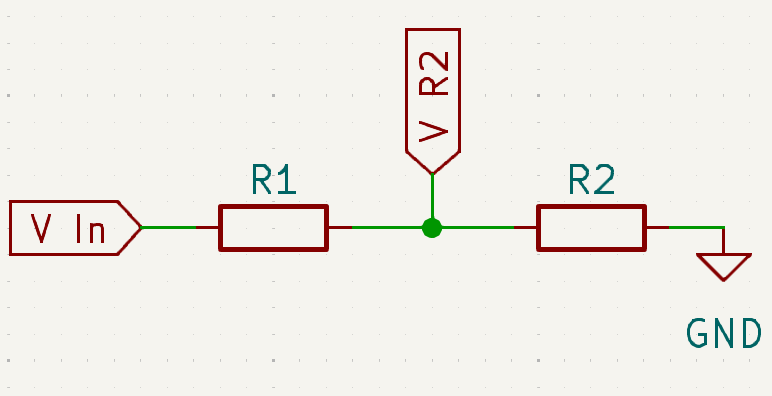
\includegraphics[width=0.6\textwidth]{figures/fig_voltage_divider.png}
    \caption{Simple voltage divider circuit used for resistance measurement.}
\end{figure}

Equations \ref{eqn:voltage_divider} and \ref{eqn:resistance_divider} are used to calculate the resistance from the voltage divider equation.
\begin{equation}\label{eqn:voltage_divider}
    V_{R2} = V_{In} \times \frac{R_2}{R_1 + R_2}
\end{equation}
\begin{equation}\label{eqn:resistance_divider}
    R_2 = \frac{R_1 \times V_{R2}}{V_{In}-V_{R2}}
\end{equation}


\section{Circuit Design}
\subsection{Probe Circuit}
The probe circuit is the circuit which contains the resistor divider, was designed to be printed onto a \gls{pcb}.
This design was influenced by Reference~\cite{cam_clark}, where a similar device was designed for salinity measurements in ice columns.
A \gls{pcb} was chosen for this circuit as the researcher had significant experience with \gls{pcb} design, and the manufacturing process offered higher precision than hand soldering, and is relatively cost-effective.
Significant improvements and modifications were made to the resistor divider circuit, to allow for a wider range of testing.

For input power, a \gls{dac} was used to drive the circuit. This allowed to the input voltage to be varied between $0 V$ and the referencevoltage, which was chosen to be $5V$.
This allowed for a range of voltages to be applied, which allowed for the measurement of the water's voltage-resistance relationship, and the creation of \gls{ac} signals.
A function generator was considered for generating the \gls{ac} signal, as it would allow for signals of a wider frequency and and high precision, however the price could not be accomodated by the budget.
The choice of \gls{dac}, and all following components, was first influenced by availability on JLCPCB, the \gls{pcb} manufacturing house.
The MCP4725 was chosen for its high resolution of 12-bits, offering a digital range of 0-4095, fast update time of $6{\mu}s$, and interface speed of 3.4MHz.
These features allow for both \gls{dc} and \gls{ac} signal analysis.

An op-amp with unity gain was the connected to the output of the \gls{dac}.
This is because \gls{dac}s have limited output drive capabilities, and the op-amp would allow for heavier loads to be driven.
Additionally the op-amp offers improved output stability, introduces impedance isolation, which protects the \gls{dac} from load variations and feedback effects, and allows for better sine wave quality.

As mentioned in Section~\ref{sec:res_mes}, for the resistor divider circuit, the electrodes would serve as R2 and a known resistor as R1.
Three alernative values of R1 were chosen, to accomodate for any circuit errors.
These could be switched between using the TS3A4751 multiplexer \gls{ic}.
This switching multiplexer was chosen, for its low on-state resistance of $0.9\Omega$, and fast switching speed of $4-5ns$~\cite{cam_clark}.

The R1 resistor values were chosen to be $100\Omega$, $1K\Omega$ and $10K\Omega$.
These values would be used when the resistance between the probes was $1-10\Omega$, $10-100\Omega$, and $100-1K\Omega$ respectively.
Each \gls{ic} contained 4 switches.

For measuring the output resistor, the voltage over it was directed into a multiplying op-amp with a gain of 11.
This increases the resolution for the \gls{adc} readings, as low voltages may be hard to differentiate between when converted to digital data. 

This configuration would allow for a minumum resolution of $11\%$ of $V_{DAC}$ and maximum of $100\%$ of $V_{DAC}$, for the voltage measurement by the \gls{adc}, as shown in Equations~\ref{eqn:dac_11} and~\ref{eqn:dac_100}~\cite{cam_clark}.
Equations~\ref{eqn:dac_11} and~\ref{eqn:dac_100} show for the expected resistance of $7.55\Omega$ falling into the $1-10\Omega$ range.
However, if the resistance falls into the $10-100\Omega$, or $100-1K\Omega$, the respective R1 resistors would be used and the maximum and minimum \gls{dac} resolutions would be the same.

\begin{equation}\label{eqn:dac_11}
    \frac{1\Omega}{1\Omega + 100\Omega}\times V_{DAC} \times 11 = 11\% V_{DAC}
\end{equation}

\begin{equation}\label{eqn:dac_100}
    \frac{10\Omega}{10\Omega + 100\Omega}\times V_{DAC} \times 11 = 100\% V_{DAC}
\end{equation}

The accuarcy of the R1 resistor is integral to acheiving an accurate R2 measurement.
The resistors available on JLCPCB had an acurracy of $\pm{1}\%$.
To increase the accuracy 3 equal resistors were put in parallel. This decreases the uncertainty of the total equivalent resistance~\cite{cam_clark}.
This is shown in Equations~\ref{eqn:parallel_r} to~\ref{eqn:parallel_uncertainty}.

\begin{equation}\label{eqn:parallel_r}
    R_{Equivalent} = {\left[{\sum_{i=1}^{n}{\frac{1}{R_n}}}\right]}^{-1}
\end{equation}
If all the Resistors are equal this simplifies to: 
\begin{equation}\label{eqn:parallel_r_equal}
    R_{Equivalent} = ({\frac{n}{R}})^{-1} = \frac{1}{n} \times R
\end{equation}
To propogate uncertainty the standard equation for combined uncertainty can be used:

If a quantity $y$ depends on several independent variables $x_1, x_2, ..., x_n$: \\
$y=f(x_1, x_2, ..., x_n)$ \\
and each $x_i$ has a standard uncertainty $u(x_i)$ then the combined standard uncertainty of $y$, denoted $u_c(y)$, is:
\begin{equation}\label{standard_uncertainty}
    u_c(y)=\root{\sum_{i=1}^{n}{({\frac{\partial{f}}{\partial{x_i}}}{u(x_i)})}^2}
\end{equation}

\chapter{Testing and Evaluation}

To properly evaluate the system, multiple testing procedures were implemented.
These started with first testing the accuarcy of individual components on the \gls{pcb}, and then testing the probes ability to measure salinity, through voltage measurements relating to conductivity.
Additionally, tests were done on the \gls{ml} model programmed to map the salinity.

A summary of the tests and their outcomes can be seen in Table~\ref{table:test_summary}. %TODO


\section{Component and Equipment Testing}
Before the probe could be used to measure salinity, the accuarcy of its components needed to be tested.
These procedures were completed before the probe was encased in resin, as access to the circuitry was required.

\subsection{Resistor Testing}
For accurate electrode resistance to be measured, the the $R1$ parallel resistor combinations would need to be measured.
As shown in Section~\ref{sec:circuit_design}, by calculation, the $R1$ resistors should have equivalent resistances of $100\Omega$, $1K\Omega$ and $10K\Omega$, with an uncertainty of $\pm0.33\%$.
These were measured using the $Keysight Technologies U3401A$ multimeter, which had a resistance accuracy of $0.1\%$.
This multimeter would be used for all subsequent \gls{dc} voltage measurements, and has a voltage accuracy of $0.02\%$.
The multimeter probes had a resistance of $0.154\Omega$ which was accounted for.
The $R1$ resistors were measured and are shown in Table~\ref{table:resistance_test}.


\begingroup
    \renewcommand{\arraystretch}{1.8} % increase row height (adjust factor as needed)
    \begin{table}[h!]
        \centering
            \begin{tabular}{|>{\centering\arraybackslash}p{5cm}|
                >{\centering\arraybackslash}m{5cm}|}
            \hline
            Theoretical R ($\Omega$) & Meausured R ($\Omega$) \\ \hline
            $99.67-100.33$ & $99.888$ \\ \hline
            $996.7-1003.3$ & $1000.146$ \\ \hline
            $9967-10033$ & $10005.746$ \\ \hline
            \end{tabular}
        \caption{Table of $R_1$ resistor measurements}
        \label{table:resistance_test}
    \end{table}
\endgroup

The calibration resistor with an expected resistance of $5\Omega\pm0.25\%$ was measured to have a resistance of $5.142\Omega$.
Taking into account the probe resistance, the calibration resistor had a resistance of $4.988\Omega$.

\subsection{DAC and ADC Accuracy}
Both the accuracy of the \gls{dac} and \gls{adc} needed to be measured as these were used for the output and measurement, respectively.

The first test was done by programming the \gls{dac} to output from its minimum to maximum value.
This would allow for the evaluation of the \gls{dac}s output offset and gain to be measured.
The \gls{adc}s were also used to measure the output of the \gls{dac}, and these measurements were compared relative to the voltage measured by the multimeter.
Figure~\ref{fig:dac_test} shows the relationship between the voltage inputted to the \gls{dac}, and its output voltage, with the output measured on the multimeter.
Note that the reference voltage of the \gls{dac} was measured to be $5.001V$.

\begin{figure}[H]\label{fig:dac_test}
    \centering
    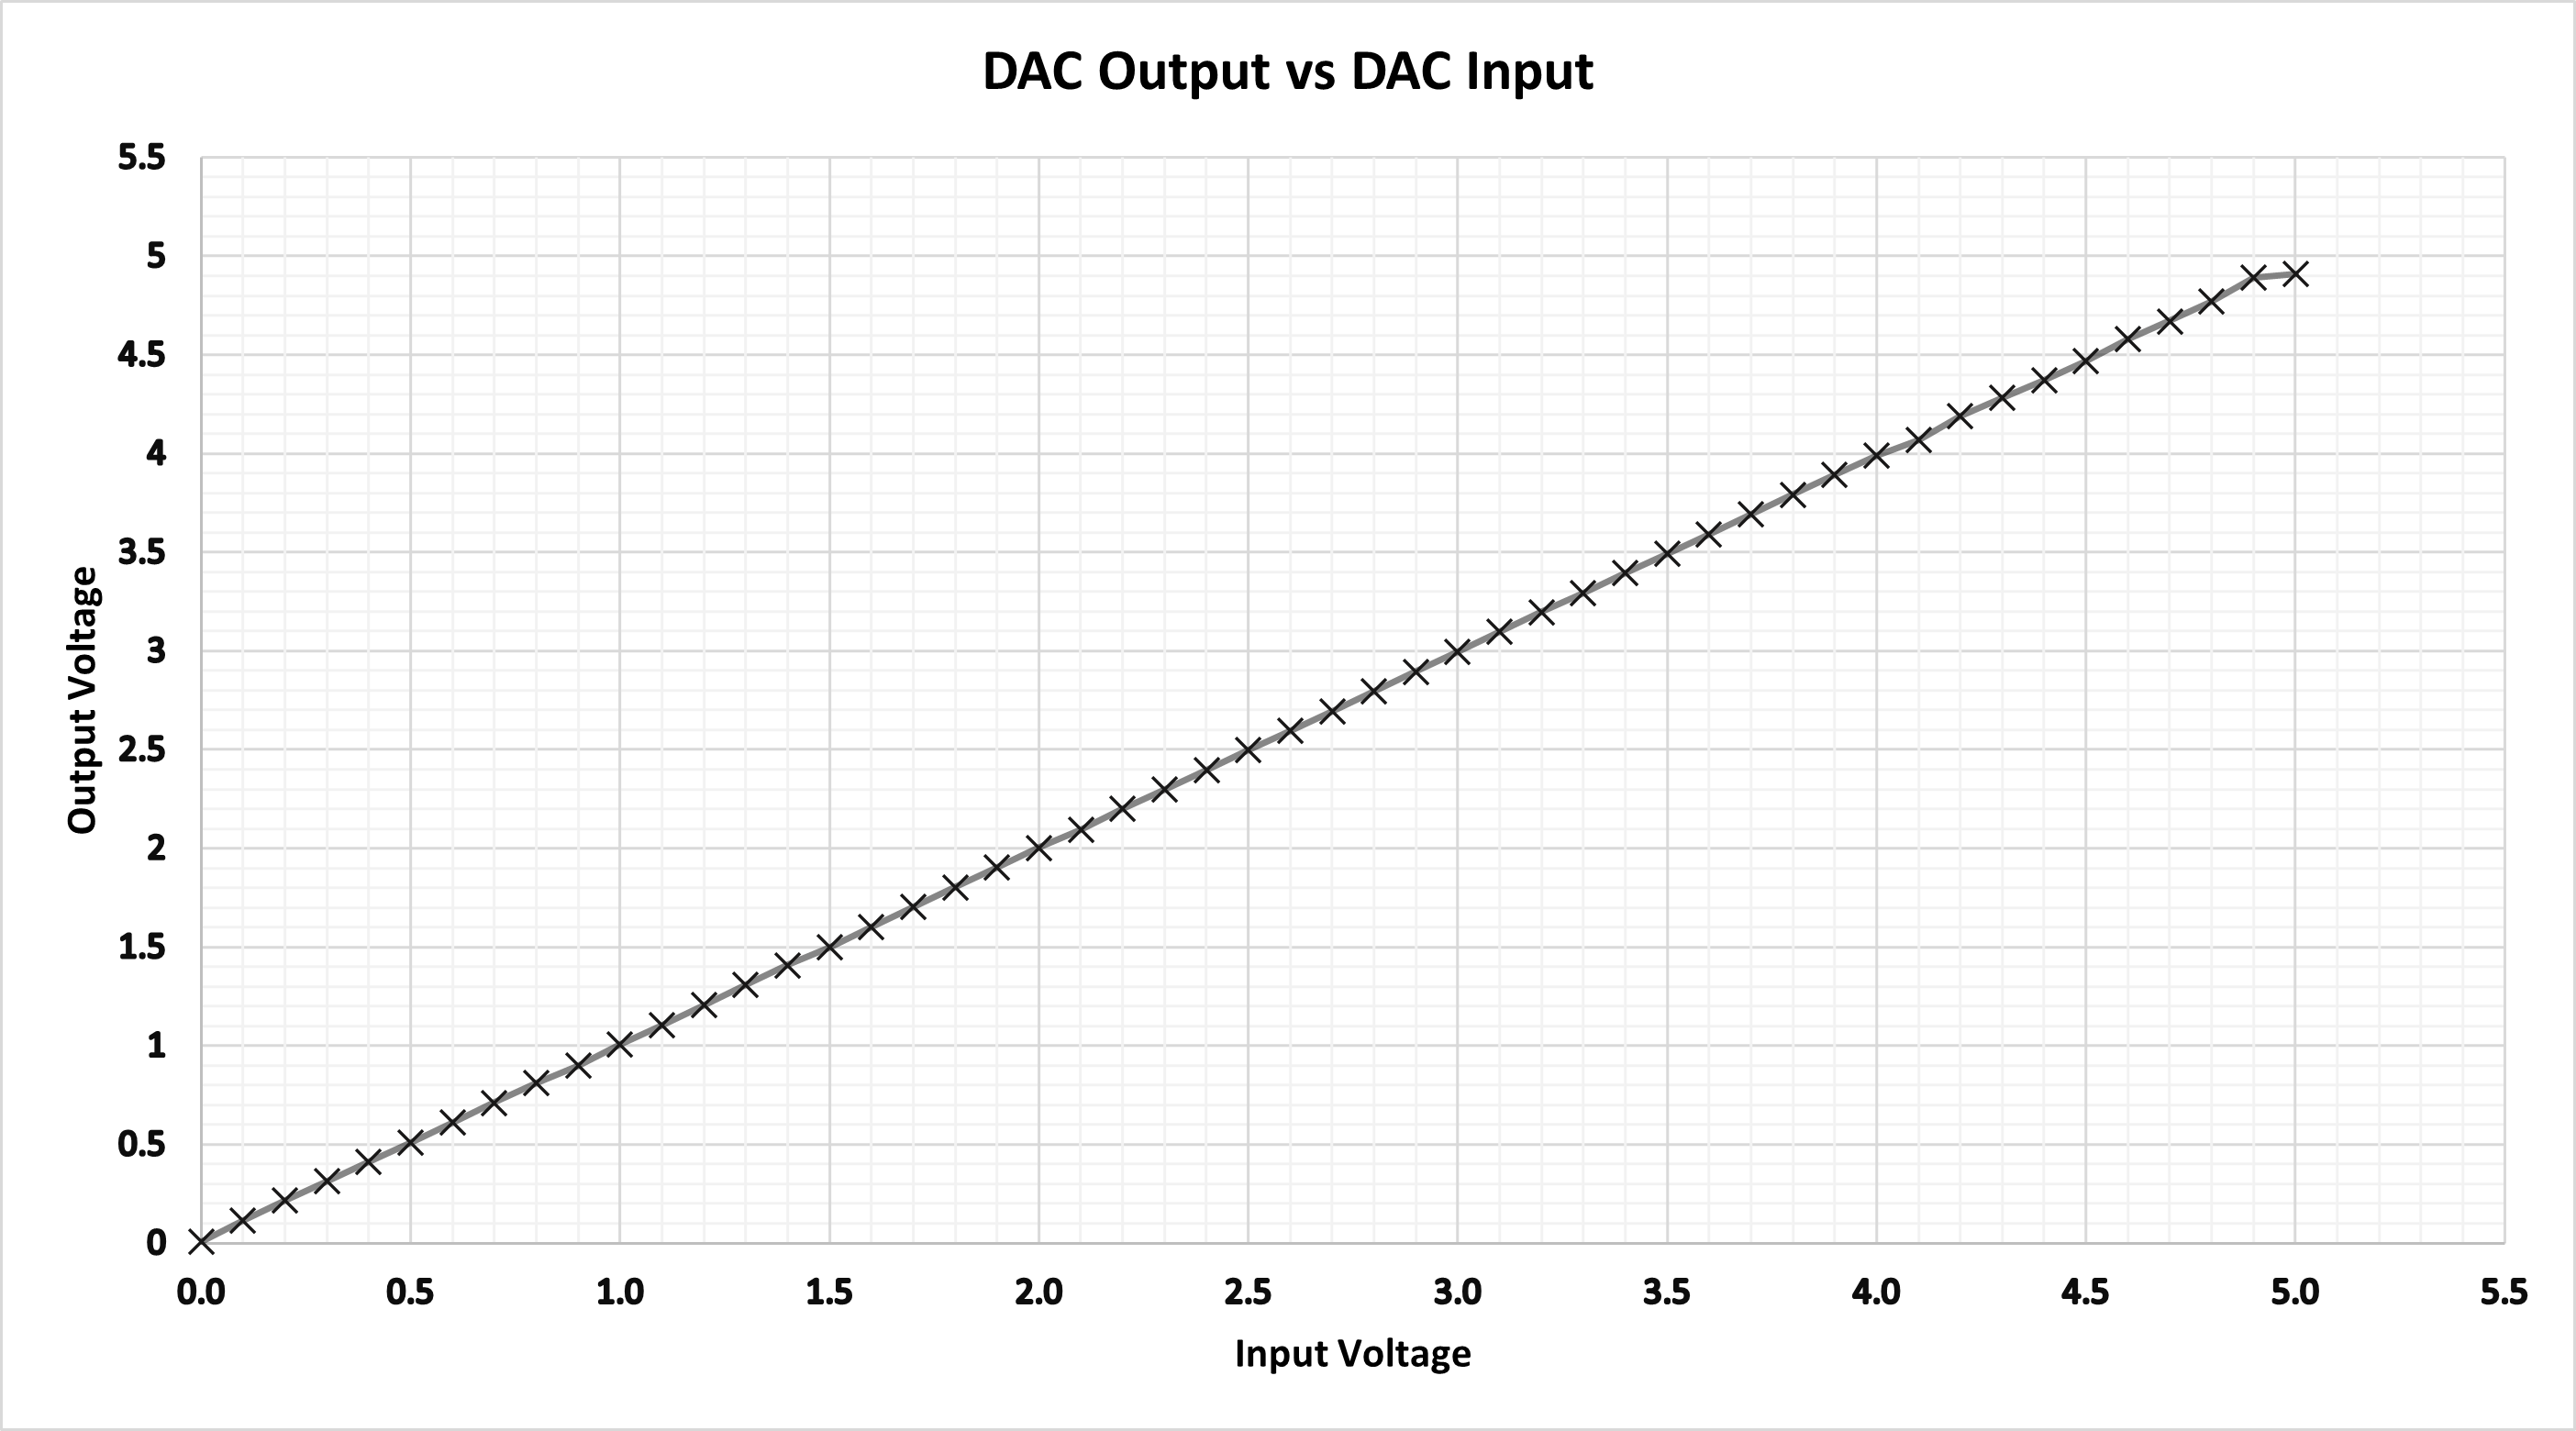
\includegraphics[width=0.7\textwidth]{figures/dac_test.png}
    \caption{DAC Output Voltage vs Input Voltage}
    \label{fig:dac_test}
\end{figure}

Based on the measurements made by the multimeter, the \gls{dac} had a output range of $0.0098V - 4.91V$, an offset of $0.0098V$ and gain of $0.98688$.

The accuracy of the \gls{adc} was then tested by comparing the \gls{dac} output measured by the \gls{adc} and multimeter.
Note, this \gls{adc} measurement was taken after the unity gain buffer op-amp.
For this test, the \gls{adc} took 5 measurements at each voltage step, which were taken at $1\mu{s}$ interval. 
These 5 values were averaged to give the voltage at that step.
The results of this test can be seen in Figure~\ref{fig:adc_test}.

\begin{figure}[H]\label{fig:adc_test}
    \centering
    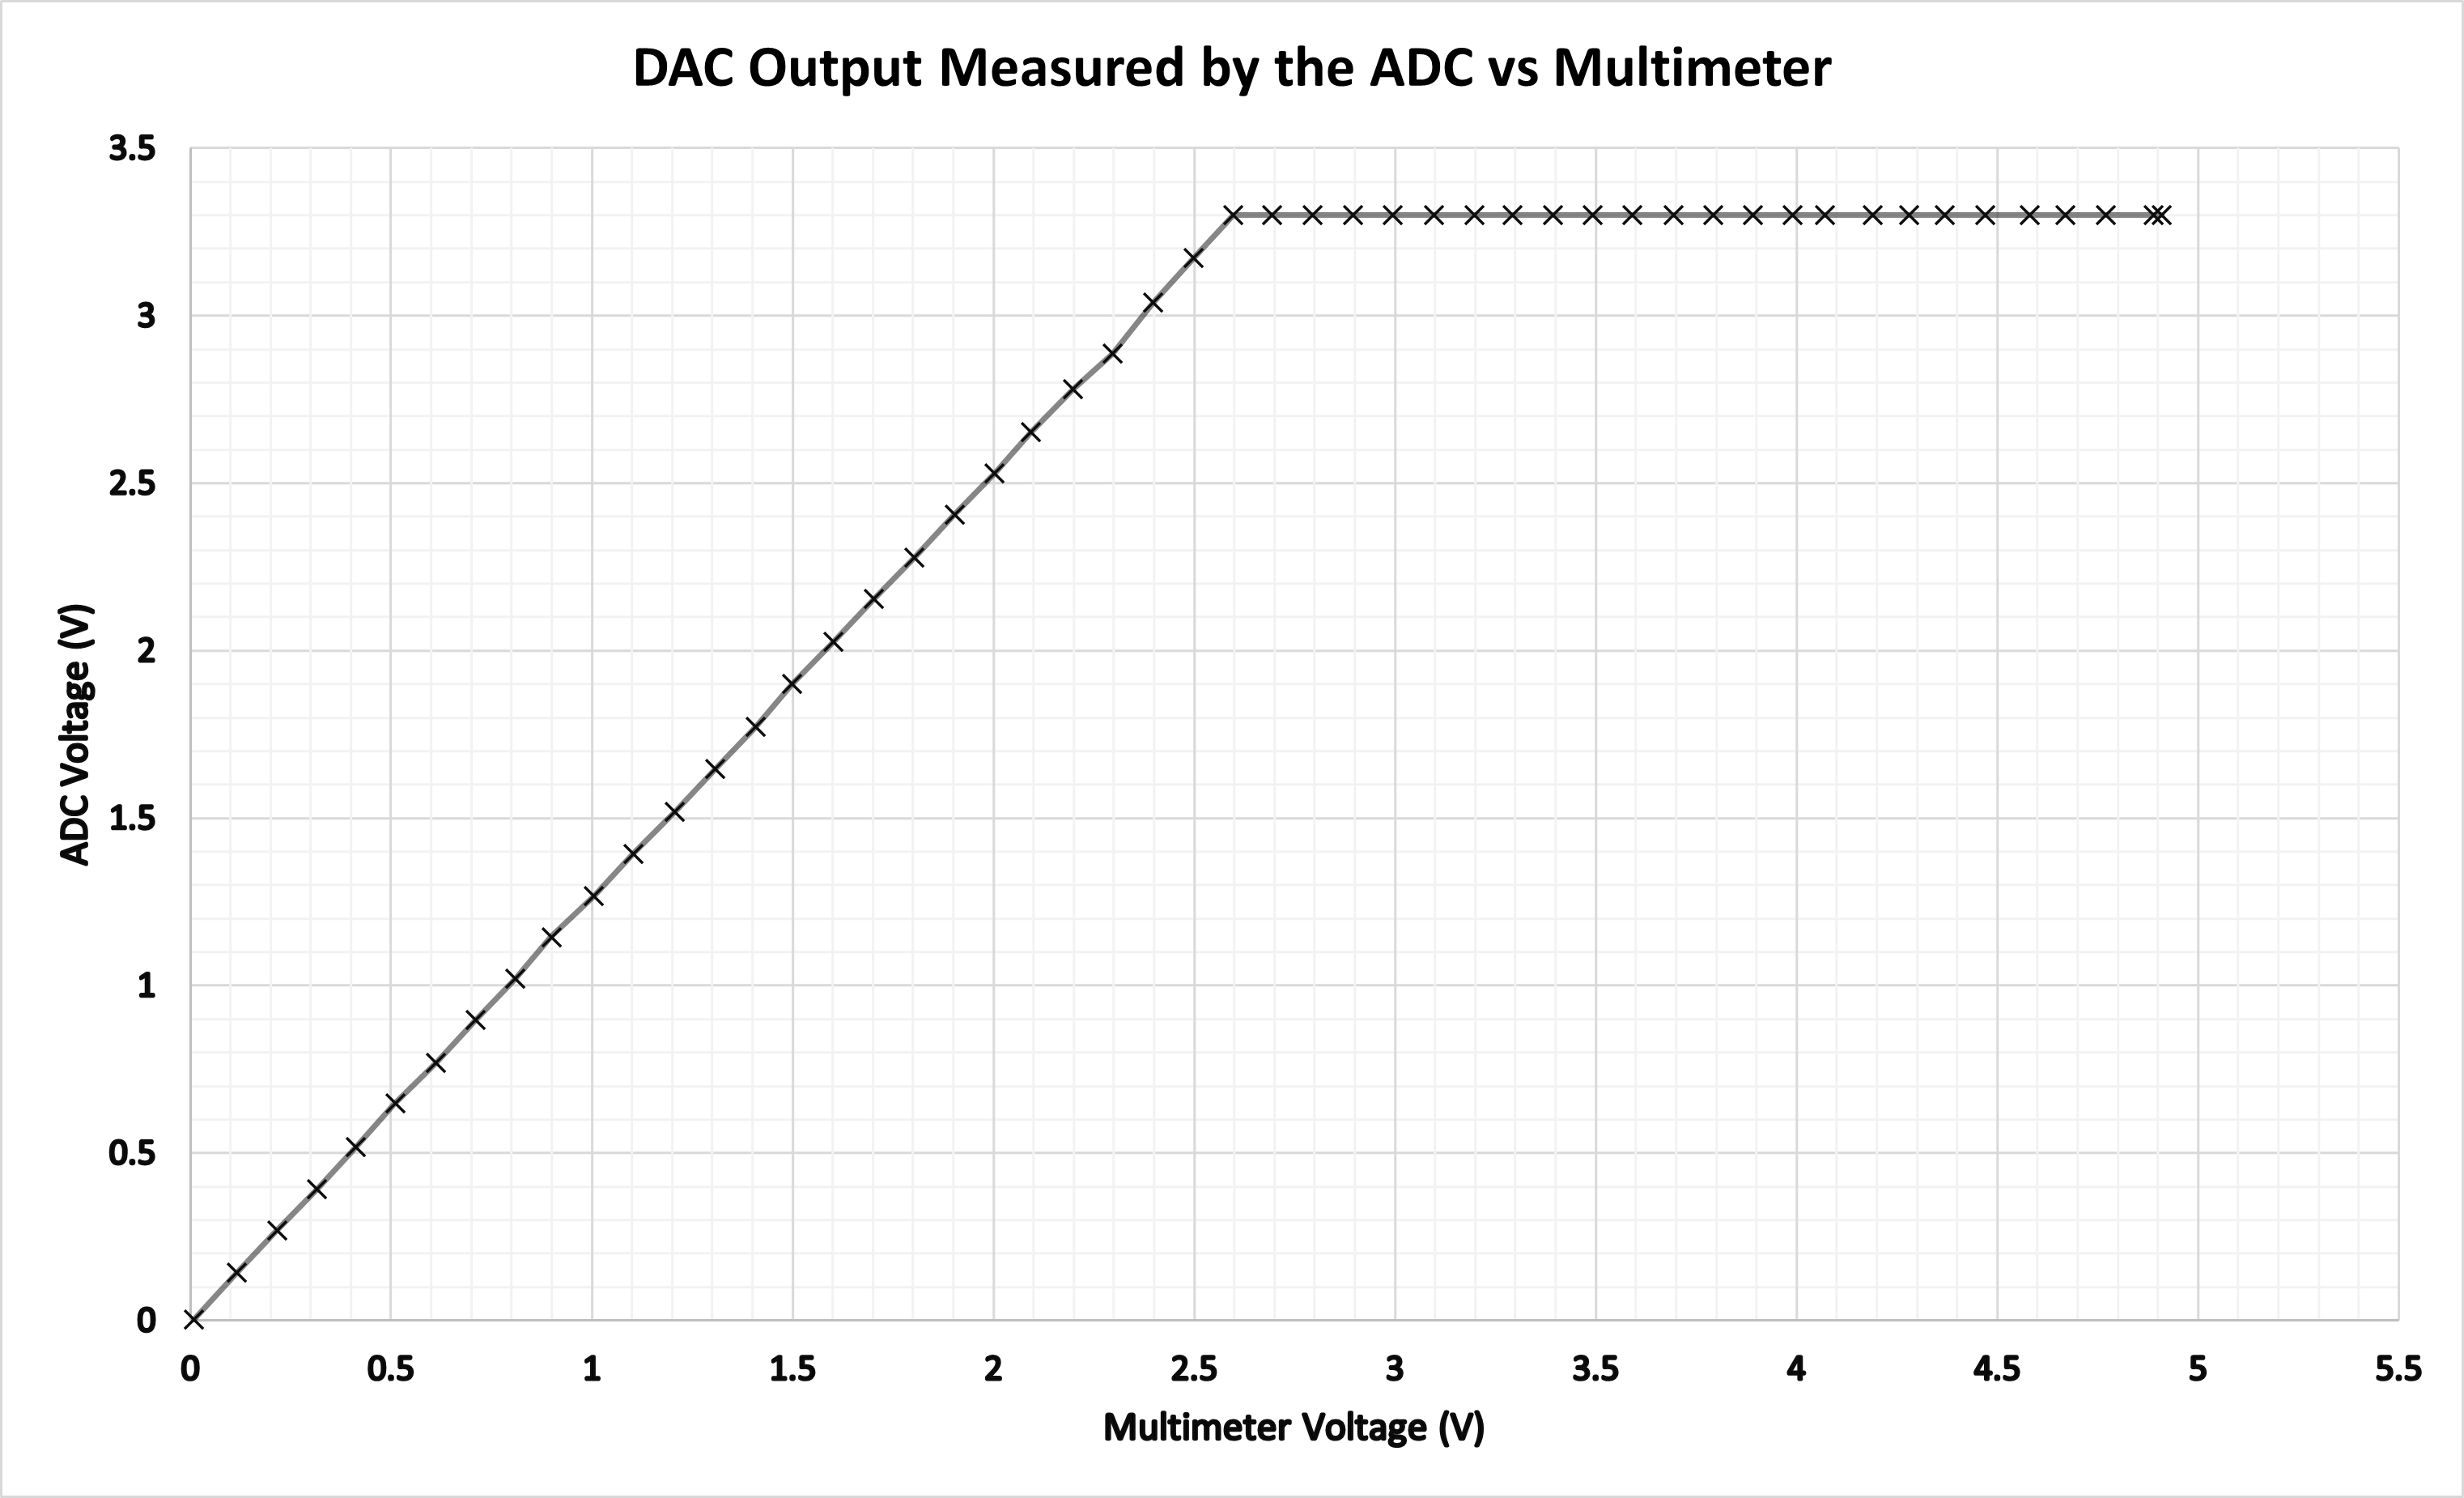
\includegraphics[width=0.7\textwidth]{figures/adc_test.png}
    \caption{DAC Output Measured by the ADC vs Multimeter}
    \label{fig:adc_test}
\end{figure}

Once the voltage measured by the \gls{adc} reaches $3.3V$ the \gls{adc} saturates as its reference voltage is $3.3V$.
The gain of the \gls{adc} was calculated to be 1.28072 compared to the mulimeter.

\subsection{Accuracy of Resistance Measuring Circuitry}\label{sec:resistor_measuring_test}
In order to evaluate the resistance circuit's ability to accurately measure resistance, resistors were attached to the electrode's solder pads.
This resistor acted as the $R2$ resistor and its value was calculated using Equation~\ref{eqn:resistance_divider}.
The resistance was calculated using the voltage sweep and single voltage functions mentioned in Section~\ref{sec:uc_program} with some slight adjustments for calculating resistance only.
These values were then compared to a multimeter measurement of the resistors, and the probe resistance taken into account.
Resistances were measured at $0\Omega$, or a short circuit, and then $10-82\Omega$ using resistors from the E12-Series, with an accuracy of $\pm5\%$
The $100\Omega$ $R1$ resistor was used.
The outcome of this test can be seen in Table~\ref{table:resistance_measurement_test}.

\begingroup
    \renewcommand{\arraystretch}{1.8} % increase row height (adjust factor as needed)
    \begin{table}[h!]
        \centering
            \begin{tabular}{|>{\centering\arraybackslash}p{4cm}|
                >{\centering\arraybackslash}m{5cm}|
                >{\centering\arraybackslash}m{6cm}|}
            \hline
                \textbf{Multimeter Resistance $\Omega$} & \textbf{Measured R $\Omega$} & \textbf{Acceptable Range $\Omega$} \\ \hline
                0 & 0 & 0-0 \\ \hline
                9.848 & 9.99578925 & 9.5-10.5 \\ \hline
                11.972 & 12.0007881 & 11.4-12.6 \\ \hline
                15.124 & 15.0062442 & 14.25-15.75 \\ \hline
                18.872 & 18.1212224 & 17.1-18.9 \\ \hline
                22.004 & 22.0162646 & 20.9-23.1 \\ \hline
                27.101 & 26.9989572 & 25.65-28.35 \\ \hline
                33.012 & 33.0181212 & 31.35-34.65 \\ \hline
                39.201 & 39.0305398 & 37.05-40.95 \\ \hline
                47.100 & 47.0431559 & 44.65-49.35 \\ \hline
                56.023 & 56.0306769 & 53.2-58.8 \\ \hline
                68.014 & 68.0599057 & 64.6-71.4 \\ \hline
                79.785 & 78.208607 & 77.9-86.1 \\ \hline
            \end{tabular}
        \caption{Table for Resistor Measurement Test}
        \textit{Note 1: For this test an input of 2V was used} \\
        \textit{Note 2: Accepectable range indicates resistance values due to $\pm5\%$ accuarcy}
        \label{table:resistance_measurement_test}
    \end{table}
\endgroup

The voltage sweep test, from 0-2V, achieved a similar measuring accuracy as seen in Figure~\ref{fig:resistance_measurement_test}
\begin{figure}[H]\label{fig:resistance_measurement_test}
    \centering
    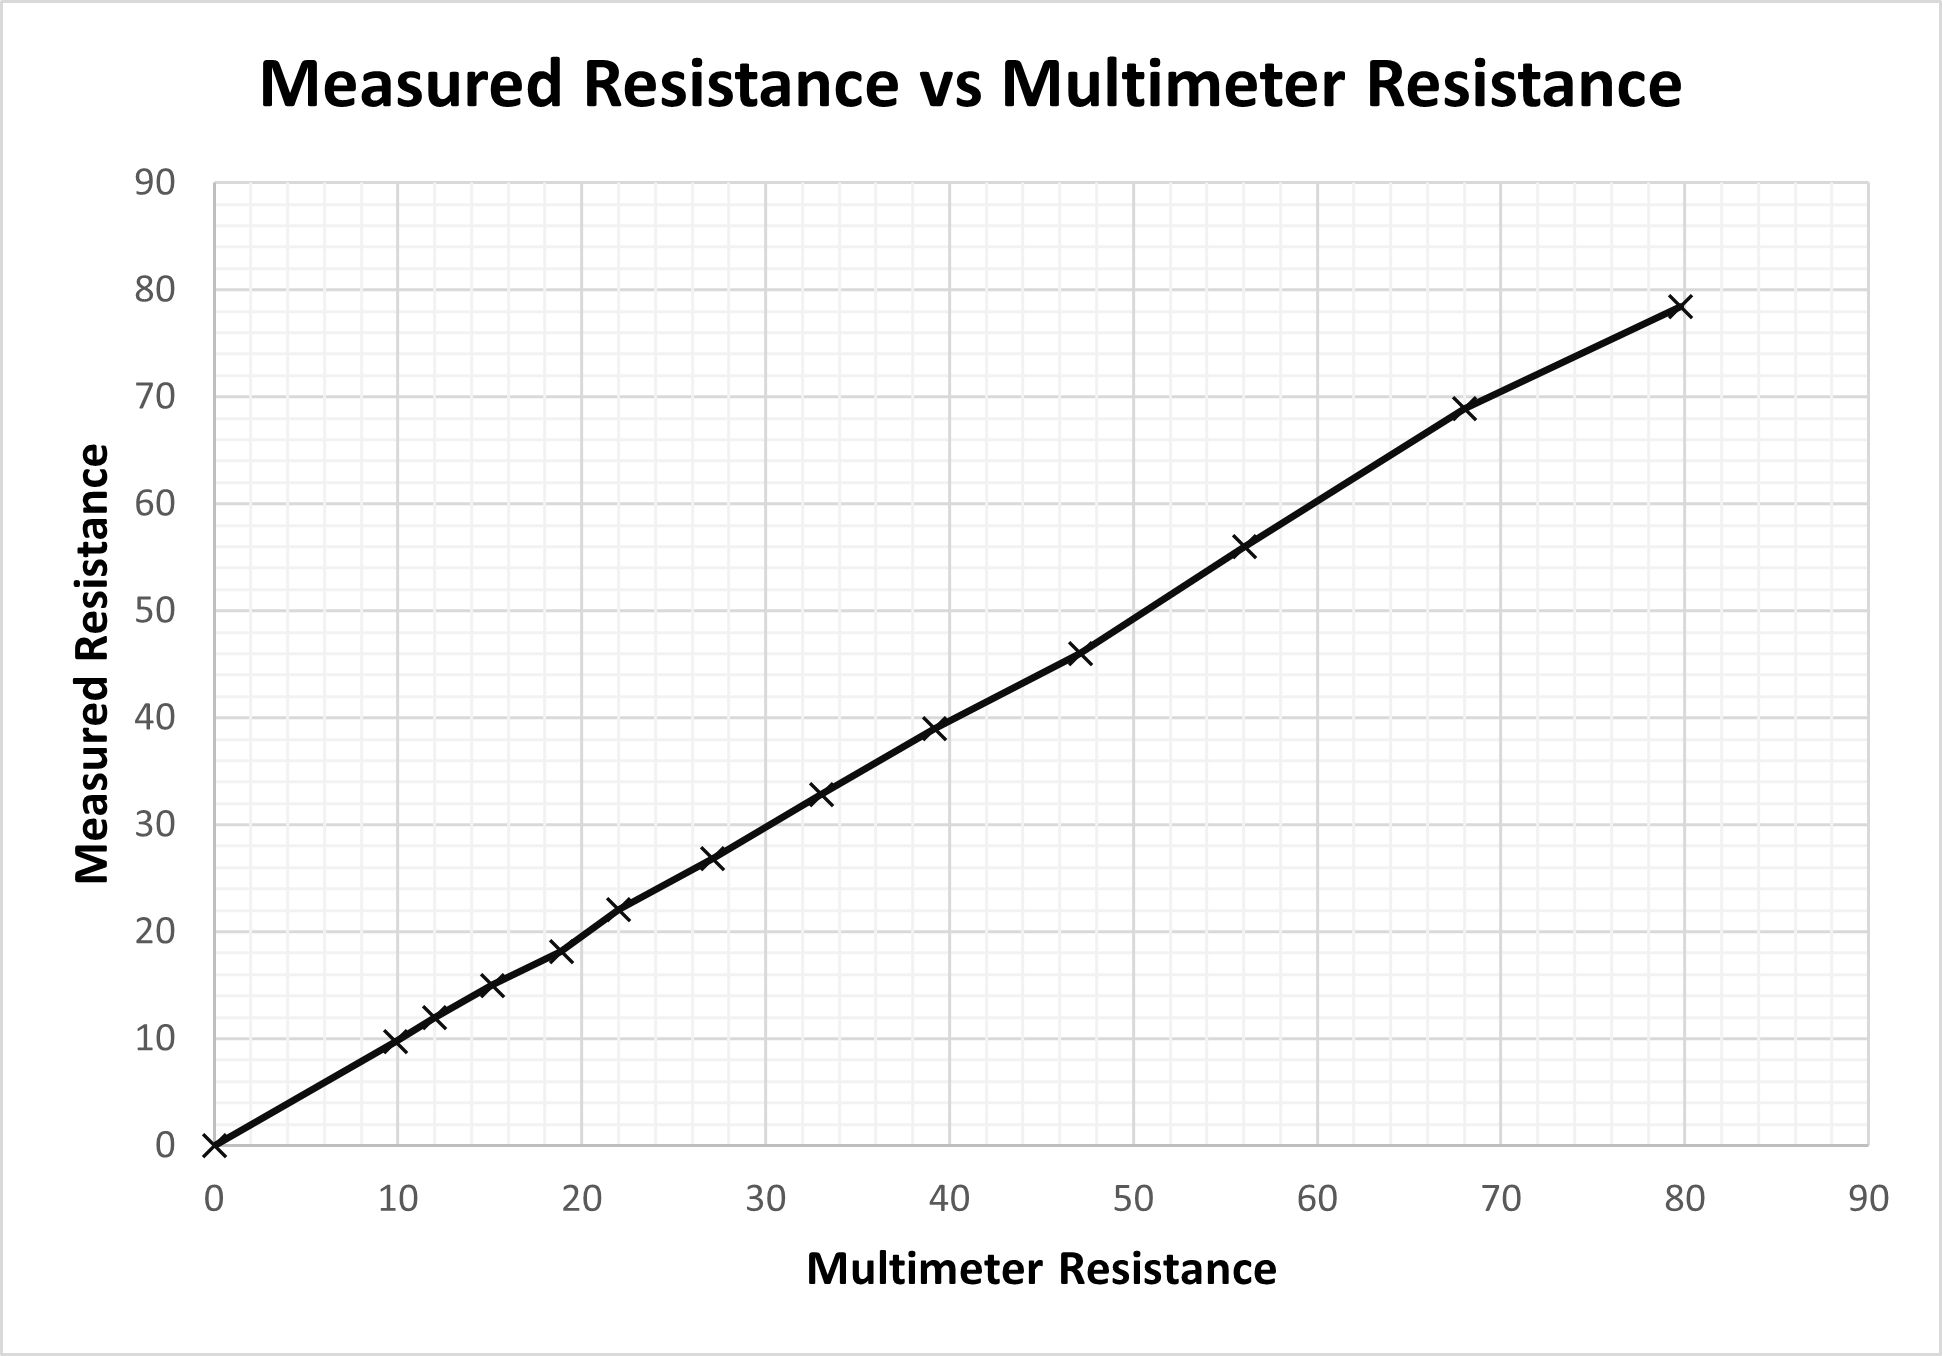
\includegraphics[width=0.7\textwidth]{figures/resistance_measurement_test.png}
    \caption{Resistance Measurement Test via Voltage Sweep}
    \label{fig:resistance_measurement_test}
\end{figure}

For both these tests, voltage calibration via the calibration resistor was done to ensure accurate voltage measurements.

\section{Salinity Testing}
In order for the probe to conduct salinity based tests, it was cast in epoxy as described in Section~\ref{sec:waterproofing}.
Following this a range of tests were conducted, ranging from testing voltage measurements on saline solutions, to measuring salinity via conductivity.

\subsection{Voltage Measurement Accuracy and Repeatability}
In order to get an understanding of how the electrodes interact with saline solutions, a voltage sweep test was conducted multiple times with the same solution.
This was done using the voltage sweep function, mentioned in Section~\ref{sec:uc_program}, with some alterations, allowing for the function to return the raw voltage instead of the conductivity.
The results showed that on the same solution, the the voltage sweep had the same effects.
However, it was noticed that when a volatge reading was taken in quick succession to another there was a slight interference was caused by the water, to counteract this a 1 second delay was introduced between each measurement.
After this delay was added, the interference was no longer observed.

Figure~\ref{fig:repeatability_test} shows voltage sweeps across the same solution on three seperate occasions.
\begin{figure}[H]\label{fig:repeatability_test}
    \centering
    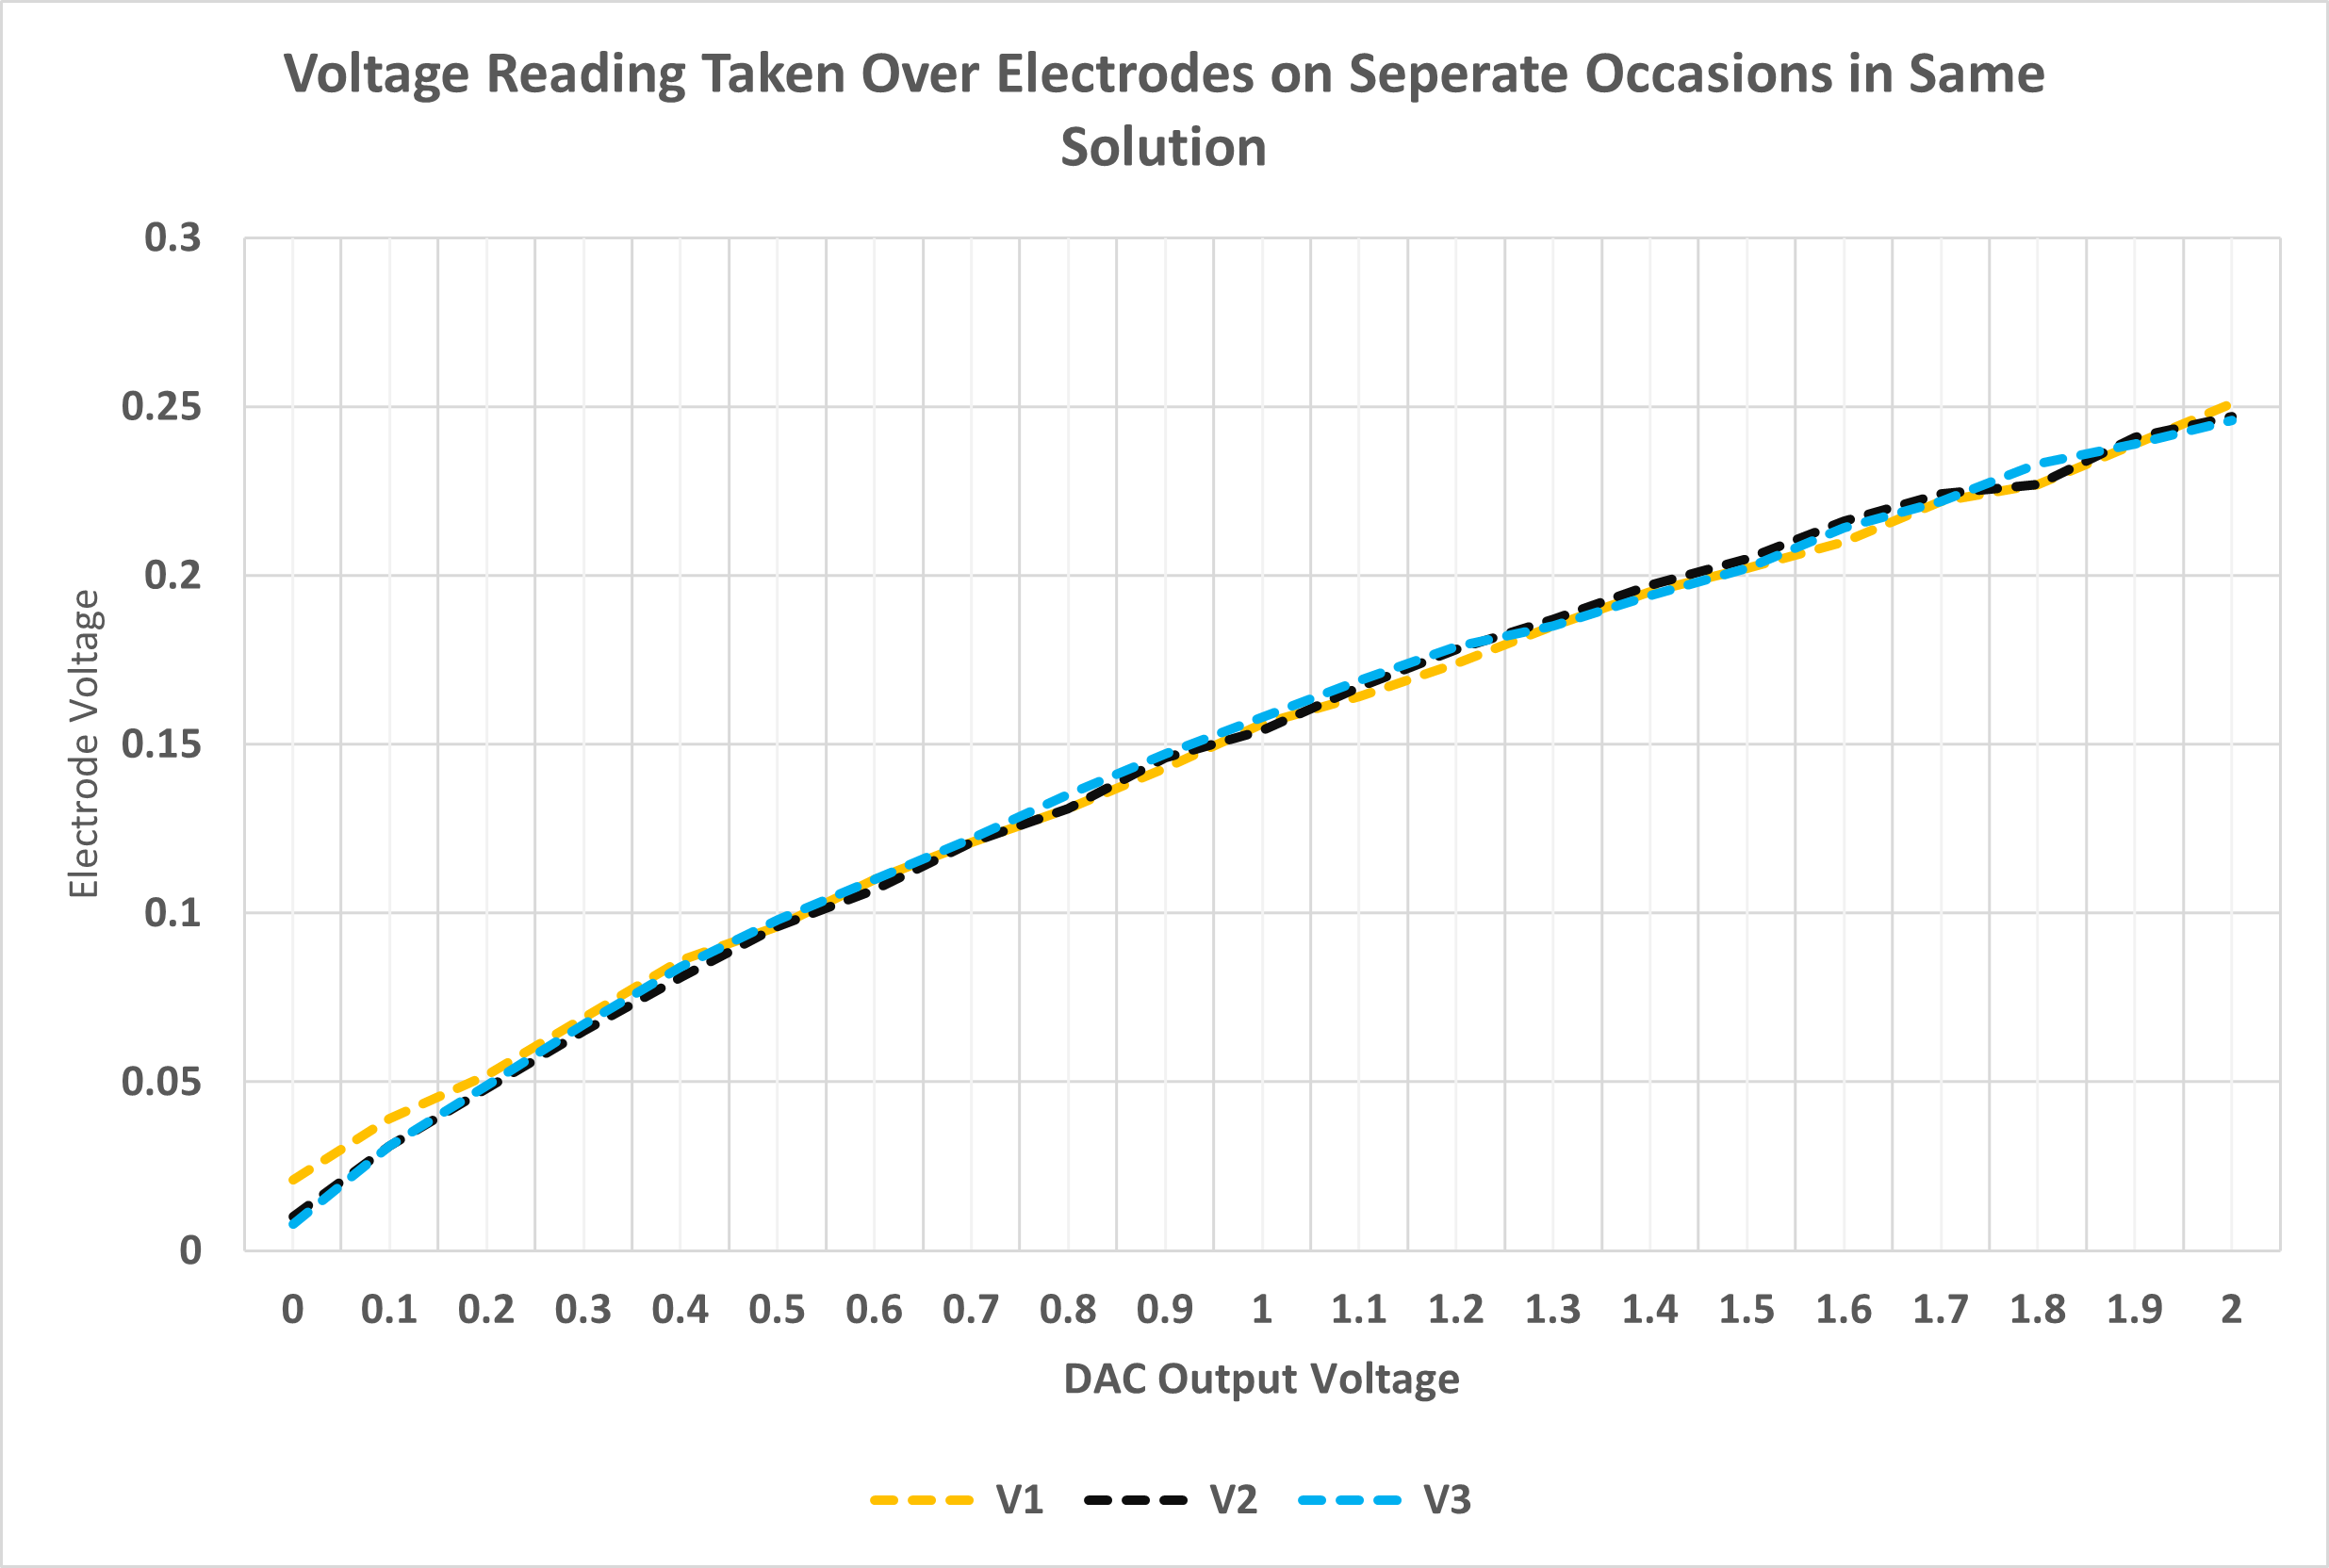
\includegraphics[width=0.7\textwidth]{figures/repeatability_test.png}
    \caption{Repeatability Test Results}
    \label{fig:repeatability_test}
\end{figure}

\subsection{Conductivity and Salinity Measurement}

\subsubsection{Obtaining Conductivity of the Standard Solution}
For the measurement of salinity from conductivity, the conductivity of the standard solution of $35$ \gls{psu} at $15^{\circ}C$ and $0dbar$ must first be obtained.
To evaluate this, both the voltage sweep and single voltage measurements wer taken in a solution at standard conditions.
To achieve these conditions salt was mied into water until the salinity was 34.8 \gls{psu}.
This value was used, as creating a solution of a specific salinity is a time-consuming process, and it was considered close enough for this experiment.
To achieve a temperature of $15^\circ$C the water was cooled in a fridge to $4^\circ$C and then left out until it reached $15^\circ$C.
The salinity was measured using a salinometer.
Once the required conditions were achieved, a voltage sweep from $0-2V$ was done using the previously mentioned voltage sweep function.
As mentioned in Section~\ref{sec:uc_program}, in the voltage sweep description, this returns the conductivity and resistance for each step.
All measurements for this and subsequent tests were conducted at $0dbar$, while using the $100\Omega$ $R_1$ resistor as the measured resistances were between $1-15\Omega$.
The sweep was conducted twice to ensure repeatability.
From this test the average conductivity of the standard solution was found to be $3.53 S/m$, with an average electrode/water resistance of $6.81\Omega$.

Similar results were obtained using single voltage measurements, where multiple readings were taken at one voltage using the DC Single Voltage function, and this was done for voltages of $1-1.5V$.
Here the average resistance was calculated to be $7.39\Omega$ and average conductivity of $3.53 S/m$.
These values correlate well with the expected resistance of $7.55\Omega$.

The Single Voltage Test can be seen in Table~\ref{table:sal_vsingledc}, with a graph illustrating the Voltage vs Resistance, taken from the Voltage Sweep Test, shown in Figure~\ref{fig:sal_vsweepdc}.

\begingroup
    \renewcommand{\arraystretch}{1.8} % increase row height (adjust factor as needed)
    \begin{table}[h!]
        \centering
            \begin{tabular}{|>{\centering\arraybackslash}p{1cm}|
                >{\centering\arraybackslash}m{1cm}|
                >{\centering\arraybackslash}m{1.8cm}|
                >{\centering\arraybackslash}m{2.2cm}|
                >{\centering\arraybackslash}m{3cm}|
                >{\centering\arraybackslash}m{3cm}|
                >{\centering\arraybackslash}m{2cm}|}
            \hline
                \textbf{V IN (V)} & \textbf{Vp AMP (V)} & \textbf{Calib F} & \textbf{Probe V (V)} & \textbf{Resistance ($\Omega$)} & \textbf{Conductivity (mS/cm)} \\ \hline
                1.2 & 1.112 & 0.7786 & 0.078709382 & 7.0195345 & 3.561489724 \\ \hline
                1.2 & 0.721 & 0.7786 & 0.051033691 & 4.4417047 & 3.628469589 \\ \hline
                1.3 & 1.355 & 0.7739 & 0.095330409 & 7.9130471 & 3.159195482 \\ \hline
                1.3 & 1.251 & 0.7739 & 0.088013536 & 7.2619240 & 3.442613812 \\ \hline
                1.4 & 1.312 & 0.7739 & 0.092305164 & 7.0586150 & 3.541770538 \\ \hline
                1.4 & 1.452 & 0.7739 & 0.102154800 & 7.8711082 & 3.176172238 \\ \hline
                1.5 & 1.573 & 0.7745 & 0.110753500 & 7.9721993 & 3.135897151 \\ \hline
                1.5 & 1.359 & 0.7745 & 0.095685955 & 6.8137148 & 3.669007482 \\ \hline
                1.6 & 2.211 & 0.7724 & 0.155525240 & 10.745988 & 3.226447904 \\ \hline 
                1.6 & 1.451 & 0.7724 & 0.101886582 & 6.8009925 & 3.675934042 \\ \hline
                \textbf{Mean} &  &  &  & \textbf{7.38991} & \textbf{3.531706371} \\ \hline
            \end{tabular}
        \caption{Table for Standard Salinity Solution Test}
        \textit{Note: For this test an R1 resistance of 100$\Omega$ was used.}
        \label{table:sal_vsingledc}
    \end{table}
\endgroup

%TODO table sweep or smth
\begin{figure}[H]\label{fig:sal_vsweepdc}
    \centering
    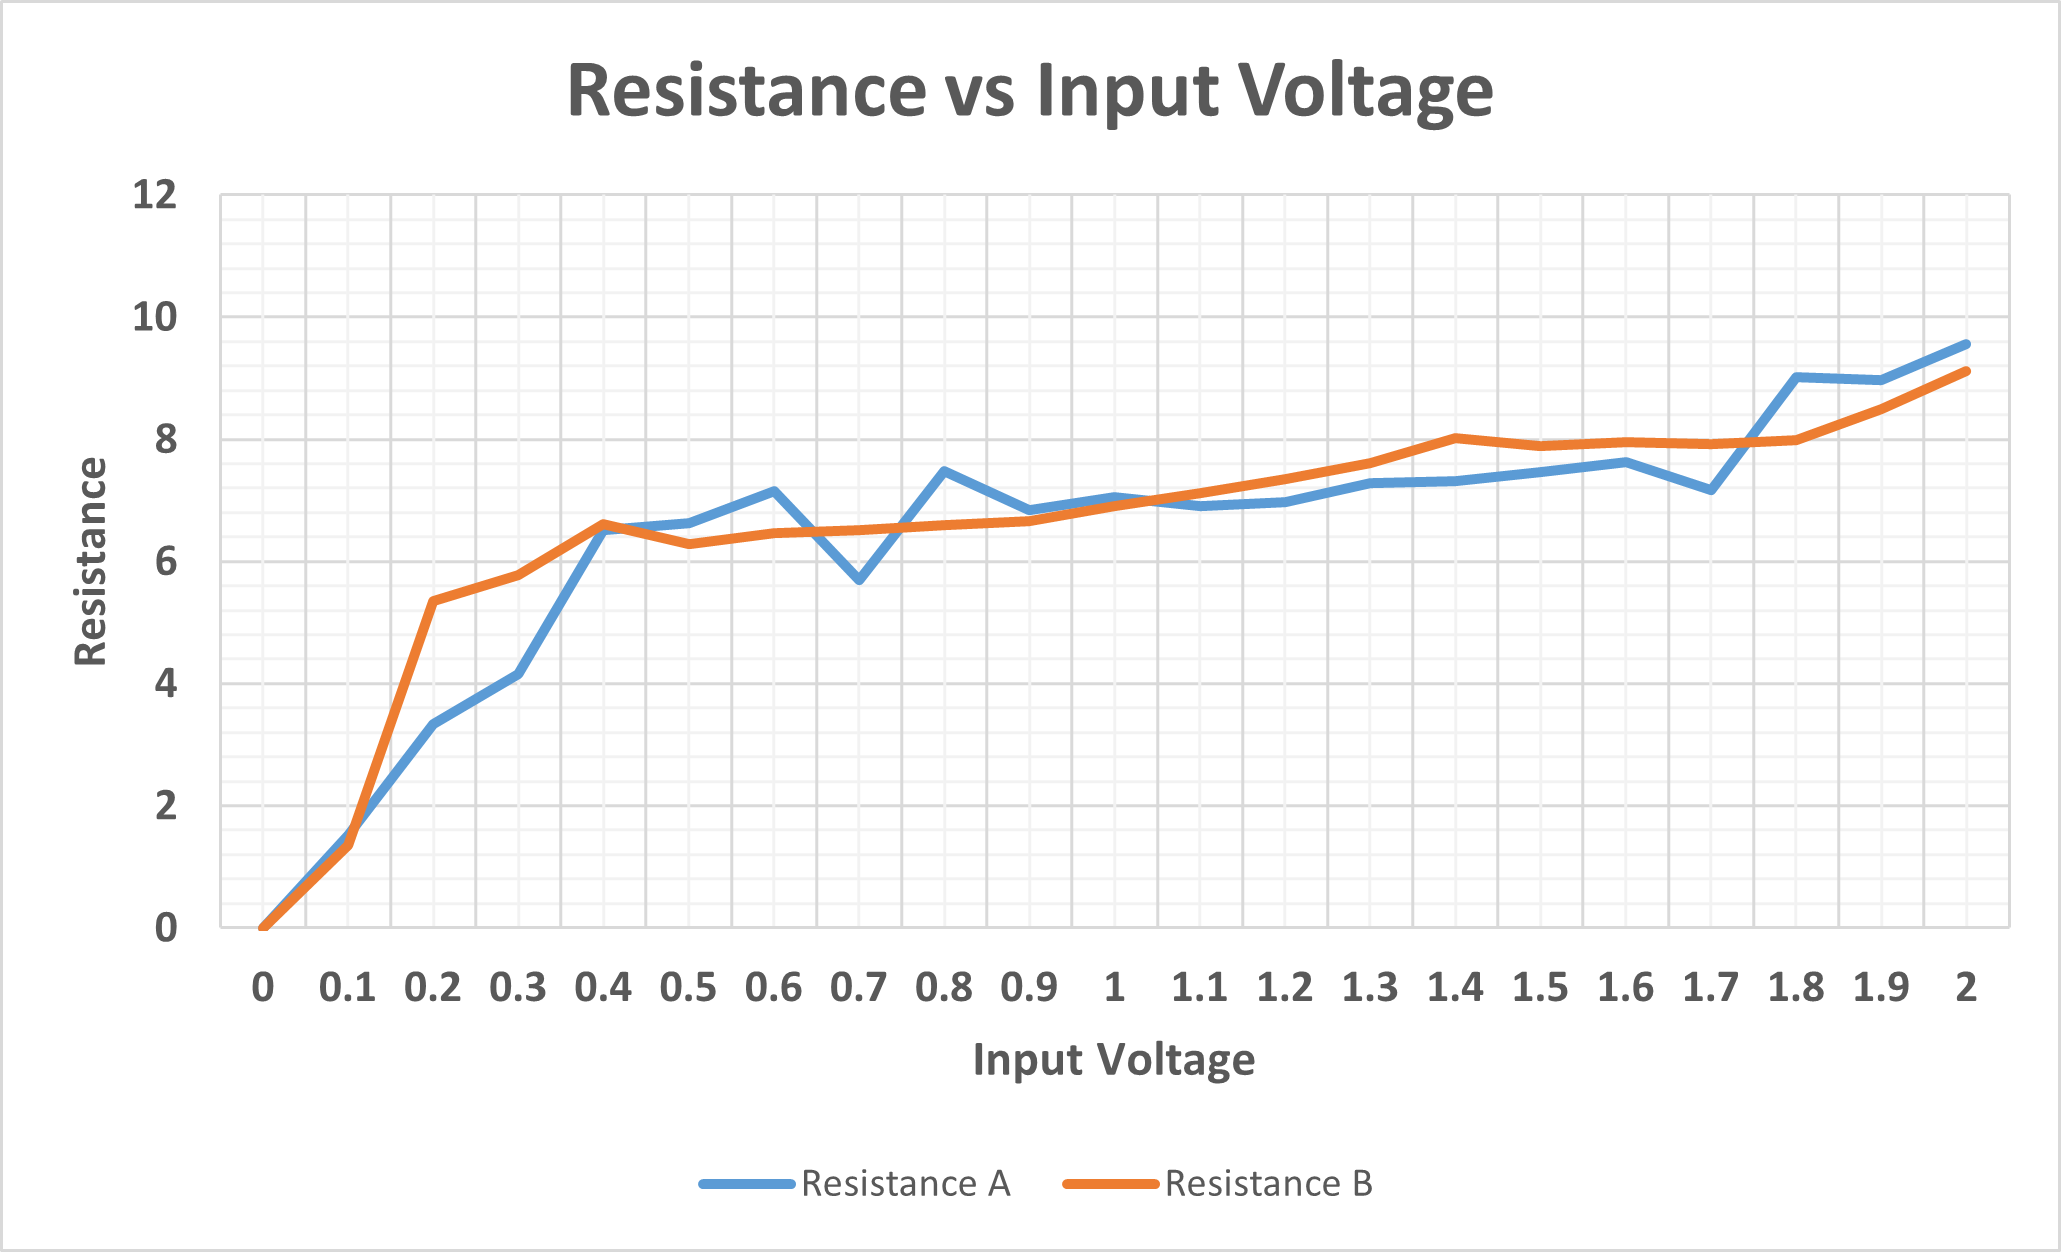
\includegraphics[width=0.7\textwidth]{figures/sal_vsweep.png}
    \caption{Volatge Sweep Test Showing Resistance vs Input Voltage}
    \label{fig:sal_vsweepdc}
\end{figure}

\subsubsection{Measuring Salinity of Sample Solutions}
Once the conductivity of the standard solution was found, the PSS-78 salinity equations could be used to find the salinity of sample solutions.
The both the DC Single Voltage and DC Sweep Voltage functions were updated to return the salinity of a measured solution.
For the DC Single Voltage Test, a voltage of $1.4V$ was found to return the most accurate value.
Using these methods salinity of solutions were tested against a salinometer and compared.
The comparisons for the Single Voltage test can be seen in Table~\ref{table:salinity_measurements}.

\begingroup
    \renewcommand{\arraystretch}{1.8} % increase row height (adjust factor as needed)
    \begin{table}[H]
        \centering
            \begin{tabular}{|>{\centering\arraybackslash}p{1.5cm}|
                >{\centering\arraybackslash}m{1cm}|
                >{\centering\arraybackslash}m{1.5cm}|
                >{\centering\arraybackslash}m{2cm}|
                >{\centering\arraybackslash}m{2.5cm}|
                >{\centering\arraybackslash}m{3cm}|
                >{\centering\arraybackslash}m{2cm}|}
            \hline
                \textbf{Salinity (PSU)} & \textbf{T (°C)} & \textbf{Probe Voltage} & \textbf{Calib Factor} & \textbf{Corrected Voltage} & \textbf{Resistance ($\Omega)$} & \textbf{Calculated Salinity} \\ \hline
                34.8  & 15    & 0.119 & 0.7739 & 0.0920941 & 7.041339901  & 35    \\ \hline
                30.1  & 15    & 0.145 & 0.7745 & 0.1123025 & 8.721186459  & 28.02 \\ \hline
                23.74 & 15    & 0.188 & 0.7601 & 0.1428988 & 11.36732667  & 20.71 \\ \hline
                23.72 & 24.31 & 0.108 & 0.7687 & 0.0830196 & 6.30378402   & 25.82 \\ \hline
                32.65 & 24.27 & 0.084 & 0.7693 & 0.0646212 & 4.839166235  & 35.15 \\ \hline
                15.8  & 20    & 0.197 & 0.7772 & 0.1531084 & 12.27920695  & 14.95 \\ \hline
                20.4  & 20    & 0.163 & 0.7779 & 0.1267977 & 9.958959389  & 18.75 \\ \hline
                17.26 & 20    & 0.197 & 0.7799 & 0.1536403 & 12.32712354  & 14.83 \\ \hline
            \end{tabular}
        \caption{Table for Sample Salinity Test}
        \textit{Note: T denotes temperature, Calib Factor denotes Calibration Factor.}
        \label{table:salinity_measurements}
    \end{table}
\endgroup

From these measured values it can be seen that the probe has a measuring accuracy of approximately $\pm3.5$ \gls{psu}.


\section{EIS and Machine Learning}
As mentioned 




\chapter{Discussion}

Here is what the results mean and how they tie to existing literature...

Discuss the relevance of your results and how they fit into the theoretical work you described in your
literature review.

\chapter{Conclusions}
This project documents the design and development of a conductivity based salinity measuring device, as well investigating the feasibility of using \gls{eis} paired with \gls{ml} to predict salinity from impedance.
It showed the successful development of a probe that used electrodes to measure conductivity, and which used conductivity, coupled with temperature and pressure, through the PSS-78 equations, to measure salinity.
It also covered the development of the controller module, used to send instructions and receive readings from the probe board. These modules both performed successfully, showing accurate salinity measurements within $\pm3.5$ \gls{psu}, and transferring data and instructions accurately.
Two methods of salinity analysis were investigated, these being \gls{dc} analysis, through resistance measuring, and \gls{ac} analysis, through \gls{eis} coupled with \gls{ml}.

The \gls{dc} analysis used two main measuring methods, a single voltage measurement, and a voltage sweep. 
These methods both return accurate resistance values, and showed good feasibility for salinity measurement.
However, further tests and investigations are required, to determine how this method can be improved.

The Resistor-Capacitor random forest model showed good prediction capabilities, with an $R^2$ value of 0,99, and optimal feature recognition. This feature recognition translated well into the salinity prediction model, were it correctly identified the features that related most to the physics of salinity.
However, this model was held back by the small dataset and low data variance, limiting its prediction capabilities.

Investigation of the effects of \gls{ac} signals on the salt water showed that it exhibited capacitive characteristics, however this needs to be tested further.

In conclusion this project showed that conductivity is a feasible method for measuring salinity, and through iteration and further development, this device can be used to measure salinity accurately.
Furthermore, the investigation into the feasibility of using \gls{eis} paired with machine learning, proved fruitful, as the models were able to learn the physics of the system.
\chapter{Recommendations}

Make sensible recommendations for further work.

%Use the IEEE numbered reference style for referencing your work as shown in your thesis guidelines.
%Please remember that the majority of your referenced work should be from journal articles, technical
%reports and books not online sources such as Wikipedia.


%Discuss the referencing style with your supervisor. When you are writing your document (if you are not using a citation editor) write the surname and date of the reference in square brackets when it is needed and highlight it as follows [Smith, 2004]. You can then return back to this later, update the numbers as they appear in text and remove the highlighting.
\cleardoublepage
\addcontentsline{toc}{chapter}{Bibliography}
\bibliographystyle{ieeetr}
\bibliography{References}

%\begin{thebibliography}{5}
%\bibitem{smt2011} M. S. Tsoeu and M. Braae, ``Control Systems,'' \emph{IEEE}, {\bf vol. 34(3)}, pp. 123-129, 2011.
%\bibitem{jct2010} J. C. Tapson, \emph{Instrumentation}, UCT Press, Cape Town, 2010.
%\end{thebibliography}

\appendix
\chapter{Proof of Graduate Attributes}

%\begin{center}
%\begin{tabular}{||p{2em} |p{15em} |p{20em}||}
% \hline
% \textbf{GA} & \textbf{Requirement} & \textbf{Justification and section in the report}  \\  [0.5ex] 
% \hline\hline
% 1 & Problem-solving & During this course I have done research on salinity measurements. This included techniques used for measuring salinity, their use cases and the mathematics behind conductivity methods used for salinity calculations. Using this research, I created a salinity measuring device that uses conductivity, temperature and depth (CTD) to measure salinity in salt water. This device required me to build a PCB and meet specific requirements, such as size and cost constraints. I had to carefully choose components and build the PCB with good practice methods used. I plan to then program this device to measure and calculate the salinity using the mathematics I researched. I have also researched Machine learning methods that can be applicable to creating a prediction or mapping model between the impedance of the salt water and its salinity. This then led to me researching Electrical Impedance Spectroscopy, which I found, should allow me to accurately create my ML model. \\  \hline
% 4 & Investigations, experiments and data analysis & I am designing a device that measures conductivity of saline solutions. Using this device, I will run an Electrical Impedance Spectroscopy measuring across the saline solution. Here I will compare the input wave to the output over the saline solution to calculate the impedance. This will be done over multiple different input waves and solutions of varying salinity to create a wide enough dataset to feed into the ML model. Here I will also use the probes to measure the salinity directly to find out the accuracy of the system and if any improvements should be made in future iterations.  \\
% \hline
% 5 & Use of engineering tools & For the hardware component of this project, I design a PCB. I used KiCAD to design both the schematic and the PCB. For the software component I plan to use VS Code and Arduino IDE with embedded C/C++. For Testing and debugging I will use tools including Oscilloscopes and Multimeters. For version control I have used Git and have a GitHub page for this project, allowing for easy changes and backing up of files. For machine learning I plan to use python with jupyter notebooks. \\
% \hline
% 6 & Professional and technical communication (Long report) & During my project I have been writing a report that documents the research I have done, the processes I have taken and my results. This report will be formatted according to the specified format and will be handed in at the end of the project. By documenting my project and meeting the deadlines I will show my ability for communication. My project also includes an oral presentation at the end which will show my presentation skills and verbal communication skills. Throughout this project I have and will submit all relevant tasks on time and have and plan to be punctual will all communication such as meetings. \\
% \hline
% 8 & Individual work & This project has shown that I have the ability to work individually, with research, design, experimentation and documentation. Where necessary I have attributed any work or ideas I have gotten from others to them. (i.e. I have referenced all sources) \\
% \hline
% 9 & Independent learning ability & have done significant research on salinity measurements, Electrical Impedance Spectroscopy, and Machine Learning algorithms. I have also designed a PCB, which involved learning about layered PCBs and interference, researching components, creating iterations to fix mistakes. This also included asking knowledgeable people such as my supervisor for advice on topics that I have some uncertainty on. \\ [1ex] 
% \hline
%\end{tabular}
%\end{center}

\begin{center}
\setlength{\extrarowheight}{1em} % optional: increases row height
\begin{longtable}{||p{2em}|p{15em}|p{20em}||}
\caption{Graduate Attributes and Justifications}\label{tab:GA_requirements} \\
\hline
\textbf{GA} & \textbf{Requirement} & \textbf{Justification and section in the report} \\ [0.5ex]
\hline
\endfirsthead

\hline
\textbf{GA} & \textbf{Requirement} & \textbf{Justification and section in the report} \\ [0.5ex]
\hline
\endhead

\hline
\multicolumn{3}{r}{\textit{Continued on next page}} \\
\hline
\endfoot

\hline
\endlastfoot

1 & Problem-solving &
During this course I have done research on salinity measurements. This included techniques used for measuring salinity, their use cases and the mathematics behind conductivity methods used for salinity calculations. Using this research, I created a salinity measuring device that uses conductivity, temperature and depth (CTD) to measure salinity in salt water. This device required me to build a PCB and meet specific requirements, such as size and cost constraints. I had to carefully choose components and build the PCB with good practice methods used. I plan to then program this device to measure and calculate the salinity using the mathematics I researched. I have also researched Machine learning methods that can be applicable to creating a prediction or mapping model between the impedance of the salt water and its salinity. This then led to me researching Electrical Impedance Spectroscopy, which I found, should allow me to accurately create my ML model. \\ \hline

4 & Investigations, experiments and data analysis &
I am designing a device that measures conductivity of saline solutions. Using this device, I will run an Electrical Impedance Spectroscopy measuring across the saline solution. Here I will compare the input wave to the output over the saline solution to calculate the impedance. This will be done over multiple different input waves and solutions of varying salinity to create a wide enough dataset to feed into the ML model. Here I will also use the probes to measure the salinity directly to find out the accuracy of the system and if any improvements should be made in future iterations. \\ \hline

5 & Use of engineering tools &
For the hardware component of this project, I design a PCB. I used KiCAD to design both the schematic and the PCB. For the software component I plan to use VS Code and Arduino IDE with embedded C/C++. For Testing and debugging I will use tools including Oscilloscopes and Multimeters. For version control I have used Git and have a GitHub page for this project, allowing for easy changes and backing up of files. For machine learning I plan to use python with jupyter notebooks. \\ \hline

6 & Professional and technical communication (Long report) &
During my project I have been writing a report that documents the research I have done, the processes I have taken and my results. This report will be formatted according to the specified format and will be handed in at the end of the project. By documenting my project and meeting the deadlines I will show my ability for communication. My project also includes an oral presentation at the end which will show my presentation skills and verbal communication skills. Throughout this project I have and will submit all relevant tasks on time and have and plan to be punctual will all communication such as meetings. \\ \hline

8 & Individual work &
This project has shown that I have the ability to work individually, with research, design, experimentation and documentation. Where necessary I have attributed any work or ideas I have gotten from others to them. (i.e. I have referenced all sources). \\ \hline

9 & Independent learning ability &
I have done significant research on salinity measurements, Electrical Impedance Spectroscopy, and Machine Learning algorithms. I have also designed a PCB, which involved learning about layered PCBs and interference, researching components, creating iterations to fix mistakes. This also included asking knowledgeable people such as my supervisor for advice on topics that I have some uncertainty on. \\ [1ex]
\hline

\end{longtable}
\end{center}

\chapter{Addenda}

\section{Ethics Forms}
}
\end{document}
